% Options for packages loaded elsewhere
\PassOptionsToPackage{unicode}{hyperref}
\PassOptionsToPackage{hyphens}{url}
%
\documentclass[
  11pt,
]{article}
\usepackage{amsmath,amssymb}
\usepackage{iftex}
\ifPDFTeX
  \usepackage[T1]{fontenc}
  \usepackage[utf8]{inputenc}
  \usepackage{textcomp} % provide euro and other symbols
\else % if luatex or xetex
  \usepackage{unicode-math} % this also loads fontspec
  \defaultfontfeatures{Scale=MatchLowercase}
  \defaultfontfeatures[\rmfamily]{Ligatures=TeX,Scale=1}
\fi
\usepackage{lmodern}
\ifPDFTeX\else
  % xetex/luatex font selection
\fi
% Use upquote if available, for straight quotes in verbatim environments
\IfFileExists{upquote.sty}{\usepackage{upquote}}{}
\IfFileExists{microtype.sty}{% use microtype if available
  \usepackage[]{microtype}
  \UseMicrotypeSet[protrusion]{basicmath} % disable protrusion for tt fonts
}{}
\makeatletter
\@ifundefined{KOMAClassName}{% if non-KOMA class
  \IfFileExists{parskip.sty}{%
    \usepackage{parskip}
  }{% else
    \setlength{\parindent}{0pt}
    \setlength{\parskip}{6pt plus 2pt minus 1pt}}
}{% if KOMA class
  \KOMAoptions{parskip=half}}
\makeatother
\usepackage{xcolor}
\usepackage[margin=1in]{geometry}
\usepackage{color}
\usepackage{fancyvrb}
\newcommand{\VerbBar}{|}
\newcommand{\VERB}{\Verb[commandchars=\\\{\}]}
\DefineVerbatimEnvironment{Highlighting}{Verbatim}{commandchars=\\\{\}}
% Add ',fontsize=\small' for more characters per line
\usepackage{framed}
\definecolor{shadecolor}{RGB}{248,248,248}
\newenvironment{Shaded}{\begin{snugshade}}{\end{snugshade}}
\newcommand{\AlertTok}[1]{\textcolor[rgb]{0.94,0.16,0.16}{#1}}
\newcommand{\AnnotationTok}[1]{\textcolor[rgb]{0.56,0.35,0.01}{\textbf{\textit{#1}}}}
\newcommand{\AttributeTok}[1]{\textcolor[rgb]{0.13,0.29,0.53}{#1}}
\newcommand{\BaseNTok}[1]{\textcolor[rgb]{0.00,0.00,0.81}{#1}}
\newcommand{\BuiltInTok}[1]{#1}
\newcommand{\CharTok}[1]{\textcolor[rgb]{0.31,0.60,0.02}{#1}}
\newcommand{\CommentTok}[1]{\textcolor[rgb]{0.56,0.35,0.01}{\textit{#1}}}
\newcommand{\CommentVarTok}[1]{\textcolor[rgb]{0.56,0.35,0.01}{\textbf{\textit{#1}}}}
\newcommand{\ConstantTok}[1]{\textcolor[rgb]{0.56,0.35,0.01}{#1}}
\newcommand{\ControlFlowTok}[1]{\textcolor[rgb]{0.13,0.29,0.53}{\textbf{#1}}}
\newcommand{\DataTypeTok}[1]{\textcolor[rgb]{0.13,0.29,0.53}{#1}}
\newcommand{\DecValTok}[1]{\textcolor[rgb]{0.00,0.00,0.81}{#1}}
\newcommand{\DocumentationTok}[1]{\textcolor[rgb]{0.56,0.35,0.01}{\textbf{\textit{#1}}}}
\newcommand{\ErrorTok}[1]{\textcolor[rgb]{0.64,0.00,0.00}{\textbf{#1}}}
\newcommand{\ExtensionTok}[1]{#1}
\newcommand{\FloatTok}[1]{\textcolor[rgb]{0.00,0.00,0.81}{#1}}
\newcommand{\FunctionTok}[1]{\textcolor[rgb]{0.13,0.29,0.53}{\textbf{#1}}}
\newcommand{\ImportTok}[1]{#1}
\newcommand{\InformationTok}[1]{\textcolor[rgb]{0.56,0.35,0.01}{\textbf{\textit{#1}}}}
\newcommand{\KeywordTok}[1]{\textcolor[rgb]{0.13,0.29,0.53}{\textbf{#1}}}
\newcommand{\NormalTok}[1]{#1}
\newcommand{\OperatorTok}[1]{\textcolor[rgb]{0.81,0.36,0.00}{\textbf{#1}}}
\newcommand{\OtherTok}[1]{\textcolor[rgb]{0.56,0.35,0.01}{#1}}
\newcommand{\PreprocessorTok}[1]{\textcolor[rgb]{0.56,0.35,0.01}{\textit{#1}}}
\newcommand{\RegionMarkerTok}[1]{#1}
\newcommand{\SpecialCharTok}[1]{\textcolor[rgb]{0.81,0.36,0.00}{\textbf{#1}}}
\newcommand{\SpecialStringTok}[1]{\textcolor[rgb]{0.31,0.60,0.02}{#1}}
\newcommand{\StringTok}[1]{\textcolor[rgb]{0.31,0.60,0.02}{#1}}
\newcommand{\VariableTok}[1]{\textcolor[rgb]{0.00,0.00,0.00}{#1}}
\newcommand{\VerbatimStringTok}[1]{\textcolor[rgb]{0.31,0.60,0.02}{#1}}
\newcommand{\WarningTok}[1]{\textcolor[rgb]{0.56,0.35,0.01}{\textbf{\textit{#1}}}}
\usepackage{longtable,booktabs,array}
\usepackage{calc} % for calculating minipage widths
% Correct order of tables after \paragraph or \subparagraph
\usepackage{etoolbox}
\makeatletter
\patchcmd\longtable{\par}{\if@noskipsec\mbox{}\fi\par}{}{}
\makeatother
% Allow footnotes in longtable head/foot
\IfFileExists{footnotehyper.sty}{\usepackage{footnotehyper}}{\usepackage{footnote}}
\makesavenoteenv{longtable}
\usepackage{graphicx}
\makeatletter
\def\maxwidth{\ifdim\Gin@nat@width>\linewidth\linewidth\else\Gin@nat@width\fi}
\def\maxheight{\ifdim\Gin@nat@height>\textheight\textheight\else\Gin@nat@height\fi}
\makeatother
% Scale images if necessary, so that they will not overflow the page
% margins by default, and it is still possible to overwrite the defaults
% using explicit options in \includegraphics[width, height, ...]{}
\setkeys{Gin}{width=\maxwidth,height=\maxheight,keepaspectratio}
% Set default figure placement to htbp
\makeatletter
\def\fps@figure{htbp}
\makeatother
\setlength{\emergencystretch}{3em} % prevent overfull lines
\providecommand{\tightlist}{%
  \setlength{\itemsep}{0pt}\setlength{\parskip}{0pt}}
\setcounter{secnumdepth}{-\maxdimen} % remove section numbering
\ifLuaTeX
  \usepackage{selnolig}  % disable illegal ligatures
\fi
\usepackage{bookmark}
\IfFileExists{xurl.sty}{\usepackage{xurl}}{} % add URL line breaks if available
\urlstyle{same}
\hypersetup{
  pdftitle={Final Project (Group 2)},
  pdfauthor={Group 2},
  hidelinks,
  pdfcreator={LaTeX via pandoc}}

\title{Final Project (Group 2)}
\author{Group 2}
\date{2024-06-02}

\begin{document}
\maketitle

\textless\textless\textless\textless\textless\textless\textless{} HEAD -
Research Question/Hypothesis: What variable in the world happiness
report (family, health, trust, generosity, and economics) has the
greatest effect on a nation's happiness score? =======

\begin{itemize}
\item
  Research Question/Hypothesis: What variable in the world happiness
  report (family, health, trust, generosity, and economics) has the
  greatest effect on a nation's happiness score?
  \textgreater\textgreater\textgreater\textgreater\textgreater\textgreater\textgreater{}
  81e6af9ac23978bbafb85c9fa12c41d73c572ee5
\item
  Hypothesis: Economics plays the largest role in a nation's happiness
  score.
\end{itemize}

\begin{Shaded}
\begin{Highlighting}[]
\FunctionTok{library}\NormalTok{(readxl)}
\FunctionTok{library}\NormalTok{(dplyr)}
\FunctionTok{library}\NormalTok{(ggplot2)}
\FunctionTok{library}\NormalTok{(tidyr)}

\NormalTok{data }\OtherTok{\textless{}{-}} \FunctionTok{read\_excel}\NormalTok{(}\StringTok{"2019.xls"}\NormalTok{)}

\FunctionTok{colnames}\NormalTok{(data)}
\end{Highlighting}
\end{Shaded}

\begin{verbatim}
## [1] "Overall rank"                 "Country or region"           
## [3] "Score"                        "GDP per capita"              
## [5] "Social support"               "Healthy life expectancy"     
## [7] "Freedom to make life choices" "Generosity"                  
## [9] "Perceptions of corruption"
\end{verbatim}

\begin{Shaded}
\begin{Highlighting}[]
\FunctionTok{library}\NormalTok{(readxl)}

\NormalTok{data }\OtherTok{\textless{}{-}} \FunctionTok{read\_excel}\NormalTok{(}\StringTok{"2019.xls"}\NormalTok{)}

\FunctionTok{print}\NormalTok{(}\FunctionTok{colnames}\NormalTok{(data))}
\end{Highlighting}
\end{Shaded}

\begin{verbatim}
## [1] "Overall rank"                 "Country or region"           
## [3] "Score"                        "GDP per capita"              
## [5] "Social support"               "Healthy life expectancy"     
## [7] "Freedom to make life choices" "Generosity"                  
## [9] "Perceptions of corruption"
\end{verbatim}

\begin{Shaded}
\begin{Highlighting}[]
\NormalTok{data }\OtherTok{\textless{}{-}}\NormalTok{ data }\SpecialCharTok{\%\textgreater{}\%}
  \FunctionTok{rename}\NormalTok{(}
    \AttributeTok{Economy =} \StringTok{\textasciigrave{}}\AttributeTok{GDP per capita}\StringTok{\textasciigrave{}}\NormalTok{,  }
    \AttributeTok{Social =} \StringTok{\textquotesingle{}Social support\textquotesingle{}}\NormalTok{,                      }
    \AttributeTok{Health =} \StringTok{\textasciigrave{}}\AttributeTok{Healthy life expectancy}\StringTok{\textasciigrave{}}\NormalTok{,}
    \AttributeTok{Freedom =} \StringTok{\textasciigrave{}}\AttributeTok{Freedom to make life choices}\StringTok{\textasciigrave{}}\NormalTok{,  }
    \AttributeTok{Corruption =} \StringTok{\textquotesingle{}Perceptions of corruption\textquotesingle{}}\NormalTok{, }
    \AttributeTok{Happiness\_Score =} \StringTok{\textasciigrave{}}\AttributeTok{Score}\StringTok{\textasciigrave{}}
\NormalTok{  )}
\FunctionTok{print}\NormalTok{(}\FunctionTok{colnames}\NormalTok{(data))}
\end{Highlighting}
\end{Shaded}

\begin{verbatim}
## [1] "Overall rank"      "Country or region" "Happiness_Score"  
## [4] "Economy"           "Social"            "Health"           
## [7] "Freedom"           "Generosity"        "Corruption"
\end{verbatim}

\begin{Shaded}
\begin{Highlighting}[]
  \FunctionTok{head}\NormalTok{(}
    \FunctionTok{select}\NormalTok{(data, Economy, Social, Health, Freedom, Corruption, Happiness\_Score)}
\NormalTok{  )}
\end{Highlighting}
\end{Shaded}

\begin{longtable}[]{@{}rrrrrr@{}}
\toprule\noalign{}
Economy & Social & Health & Freedom & Corruption & Happiness\_Score \\
\midrule\noalign{}
\endhead
\bottomrule\noalign{}
\endlastfoot
1.340 & 1.587 & 0.986 & 0.596 & 0.393 & 7.769 \\
1.383 & 1.573 & 0.996 & 0.592 & 0.410 & 7.600 \\
1.488 & 1.582 & 1.028 & 0.603 & 0.341 & 7.554 \\
1.380 & 1.624 & 1.026 & 0.591 & 0.118 & 7.494 \\
1.396 & 1.522 & 0.999 & 0.557 & 0.298 & 7.488 \\
1.452 & 1.526 & 1.052 & 0.572 & 0.343 & 7.480 \\
\end{longtable}

{[}Module 2: Junhyung Kim, Jiho Lee{]}

*Scatter Plot

\begin{Shaded}
\begin{Highlighting}[]
\FunctionTok{qplot}\NormalTok{(}\AttributeTok{x =}\NormalTok{ Economy, }\AttributeTok{y=}\NormalTok{ Happiness\_Score, }\AttributeTok{data =}\NormalTok{ data,}
 \AttributeTok{geom =} \FunctionTok{c}\NormalTok{(}\StringTok{"point"}\NormalTok{, }\StringTok{"smooth"}\NormalTok{), }\AttributeTok{method =} \StringTok{"lm"}\NormalTok{) }\SpecialCharTok{+}
 \FunctionTok{labs}\NormalTok{(}\AttributeTok{title =}
 \StringTok{"Scatter Plot of Relationship Between}
\StringTok{ Economy and Happiness Score"}\NormalTok{,}
 \AttributeTok{x =} \StringTok{"Economy"}\NormalTok{, }\AttributeTok{y =} \StringTok{"Happiness Score"}\NormalTok{)}
\end{Highlighting}
\end{Shaded}

\begin{verbatim}
## Warning: `qplot()` was deprecated in ggplot2 3.4.0.
## This warning is displayed once every 8 hours.
## Call `lifecycle::last_lifecycle_warnings()` to see where this warning was
## generated.
\end{verbatim}

\begin{verbatim}
## Warning in geom_point(method = "lm"): Ignoring unknown parameters: `method`
\end{verbatim}

\begin{verbatim}
## `geom_smooth()` using formula = 'y ~ x'
\end{verbatim}

\begin{center}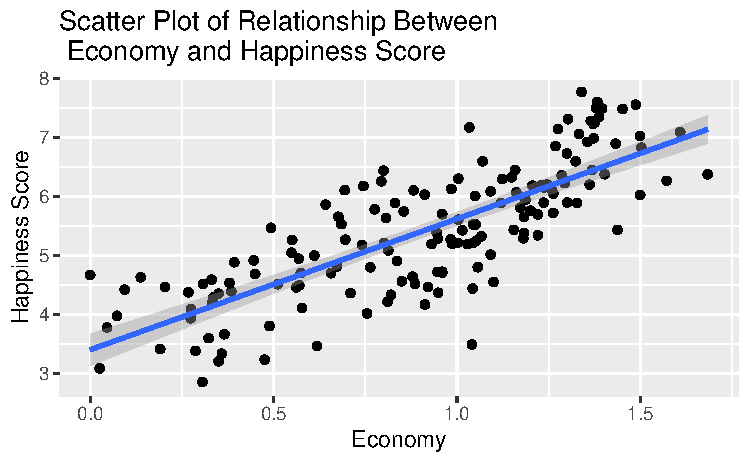
\includegraphics[width=0.7\linewidth]{Group_project_2_files/figure-latex/unnamed-chunk-4-1} \end{center}

\begin{Shaded}
\begin{Highlighting}[]
 \FunctionTok{qplot}\NormalTok{(}\AttributeTok{x=}\NormalTok{ Social,}\AttributeTok{y=}\NormalTok{Happiness\_Score,}\AttributeTok{data=}\NormalTok{data,}
 \AttributeTok{geom=}\FunctionTok{c}\NormalTok{(}\StringTok{"point"}\NormalTok{,}\StringTok{"smooth"}\NormalTok{),}\AttributeTok{method=}\StringTok{"lm"}\NormalTok{)}\SpecialCharTok{+}
 \FunctionTok{labs}\NormalTok{(}\AttributeTok{title =}
 \StringTok{"Scatter Plot of Relationship Between}
\StringTok{ Social and Happiness Score"}\NormalTok{,}
 \AttributeTok{x=}\StringTok{"Social"}\NormalTok{,}\AttributeTok{y=}\StringTok{"Happiness Score"}\NormalTok{)}
\end{Highlighting}
\end{Shaded}

\begin{verbatim}
## Warning in geom_point(method = "lm"): Ignoring unknown parameters: `method`
\end{verbatim}

\begin{verbatim}
## `geom_smooth()` using formula = 'y ~ x'
\end{verbatim}

\begin{center}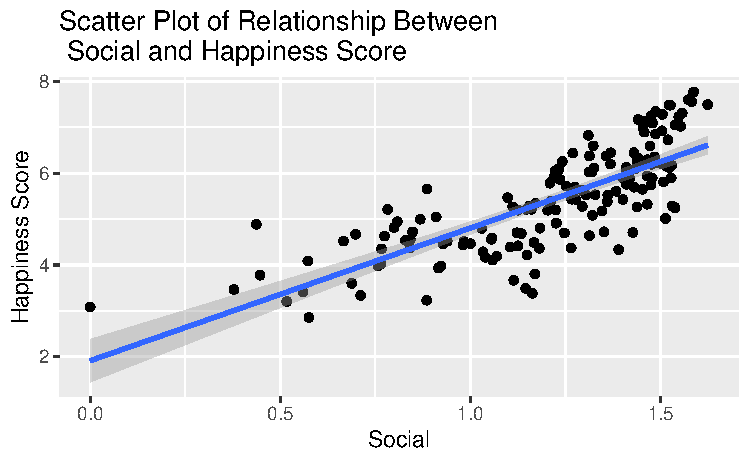
\includegraphics[width=0.7\linewidth]{Group_project_2_files/figure-latex/unnamed-chunk-5-1} \end{center}

\begin{Shaded}
\begin{Highlighting}[]
\FunctionTok{qplot}\NormalTok{(}\AttributeTok{x=}\NormalTok{ Health,}\AttributeTok{y=}\NormalTok{Happiness\_Score,}\AttributeTok{data=}\NormalTok{data,}
 \AttributeTok{geom=}\FunctionTok{c}\NormalTok{(}\StringTok{"point"}\NormalTok{,}\StringTok{"smooth"}\NormalTok{),}\AttributeTok{method=}\StringTok{"lm"}\NormalTok{)}\SpecialCharTok{+}
 \FunctionTok{labs}\NormalTok{(}\AttributeTok{title =}
 \StringTok{"Scatter Plot of Relationship Between}
\StringTok{ Health and Happiness Score"}\NormalTok{,}
 \AttributeTok{x=}\StringTok{"Health"}\NormalTok{,}\AttributeTok{y=}\StringTok{"Happiness Score"}\NormalTok{)}
\end{Highlighting}
\end{Shaded}

\begin{verbatim}
## Warning in geom_point(method = "lm"): Ignoring unknown parameters: `method`
\end{verbatim}

\begin{verbatim}
## `geom_smooth()` using formula = 'y ~ x'
\end{verbatim}

\begin{center}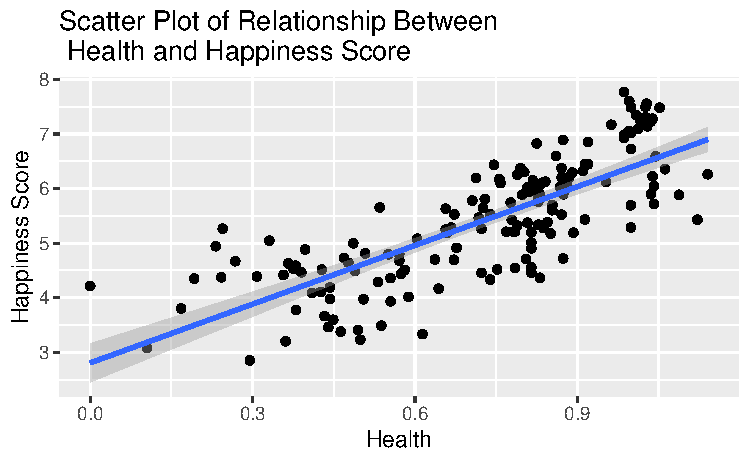
\includegraphics[width=0.7\linewidth]{Group_project_2_files/figure-latex/unnamed-chunk-6-1} \end{center}

\begin{Shaded}
\begin{Highlighting}[]
\FunctionTok{qplot}\NormalTok{(}\AttributeTok{x=}\NormalTok{ Freedom,}\AttributeTok{y=}\NormalTok{Happiness\_Score,}\AttributeTok{data=}\NormalTok{data,}
 \AttributeTok{geom=}\FunctionTok{c}\NormalTok{(}\StringTok{"point"}\NormalTok{,}\StringTok{"smooth"}\NormalTok{),}\AttributeTok{method=}\StringTok{"lm"}\NormalTok{)}\SpecialCharTok{+}
 \FunctionTok{labs}\NormalTok{(}\AttributeTok{title =}
 \StringTok{"Scatter Plot of Relationship Between}
\StringTok{ Freedom and Happiness Score"}\NormalTok{,}
 \AttributeTok{x=}\StringTok{"Freedom"}\NormalTok{,}\AttributeTok{y=}\StringTok{"Happiness Score"}\NormalTok{)}
\end{Highlighting}
\end{Shaded}

\begin{verbatim}
## `geom_smooth()` using formula = 'y ~ x'
\end{verbatim}

\begin{center}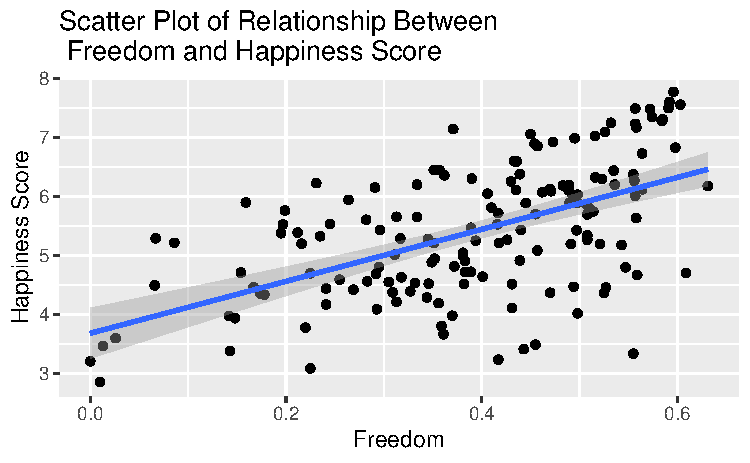
\includegraphics[width=0.7\linewidth]{Group_project_2_files/figure-latex/unnamed-chunk-7-1} \end{center}

\begin{Shaded}
\begin{Highlighting}[]
 \FunctionTok{qplot}\NormalTok{(}\AttributeTok{x=}\NormalTok{ Corruption,}\AttributeTok{y=}\NormalTok{Happiness\_Score,}\AttributeTok{data=}\NormalTok{data,}
 \AttributeTok{geom=}\FunctionTok{c}\NormalTok{(}\StringTok{"point"}\NormalTok{,}\StringTok{"smooth"}\NormalTok{),}\AttributeTok{method=}\StringTok{"lm"}\NormalTok{)}\SpecialCharTok{+}
 \FunctionTok{labs}\NormalTok{(}\AttributeTok{title =}\StringTok{"Scatter Plot of Relationship Between}
\StringTok{ Corruption and Happiness Score"}\NormalTok{,}
 \AttributeTok{x=}\StringTok{"Corruption"}\NormalTok{,}\AttributeTok{y=}\StringTok{"HappinessScore"}\NormalTok{)}
\end{Highlighting}
\end{Shaded}

\begin{verbatim}
## `geom_smooth()` using formula = 'y ~ x'
\end{verbatim}

\begin{center}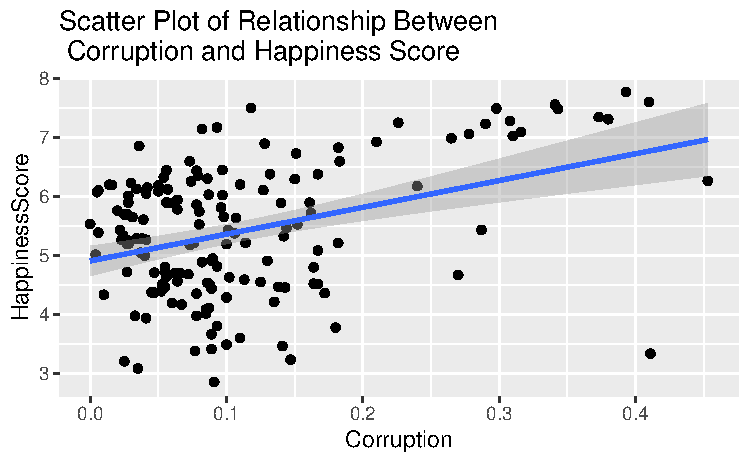
\includegraphics[width=0.7\linewidth]{Group_project_2_files/figure-latex/unnamed-chunk-8-1} \end{center}

\begin{Shaded}
\begin{Highlighting}[]
\NormalTok{data }\SpecialCharTok{\%\textgreater{}\%}
  \FunctionTok{ggplot}\NormalTok{() }\SpecialCharTok{+}
  \FunctionTok{geom\_smooth}\NormalTok{(}\AttributeTok{mapping =} \FunctionTok{aes}\NormalTok{(}\AttributeTok{x =}\NormalTok{ Economy, }\AttributeTok{y =}\NormalTok{ Happiness\_Score)) }\SpecialCharTok{+}
  \FunctionTok{labs}\NormalTok{(}\AttributeTok{x =} \StringTok{"Economy"}\NormalTok{, }\AttributeTok{y =} \StringTok{"Happiness Score"}\NormalTok{, }
       \AttributeTok{title=}\StringTok{"Trend line relationship between }
\StringTok{       Economy vs Happiness Score"}\NormalTok{)}
\end{Highlighting}
\end{Shaded}

\begin{verbatim}
## `geom_smooth()` using method = 'loess' and formula = 'y ~ x'
\end{verbatim}

\begin{center}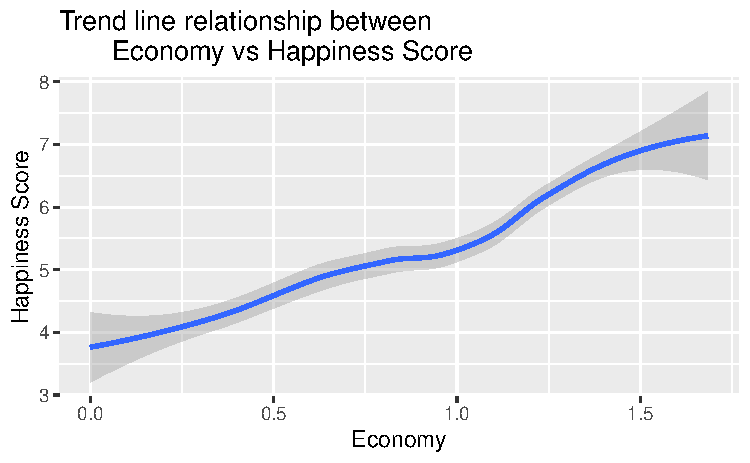
\includegraphics[width=0.7\linewidth]{Group_project_2_files/figure-latex/unnamed-chunk-9-1} \end{center}

\begin{Shaded}
\begin{Highlighting}[]
\NormalTok{data }\SpecialCharTok{\%\textgreater{}\%}
  \FunctionTok{ggplot}\NormalTok{() }\SpecialCharTok{+}
  \FunctionTok{geom\_smooth}\NormalTok{(}\AttributeTok{mapping =} \FunctionTok{aes}\NormalTok{(}\AttributeTok{x =}\NormalTok{ Social, }\AttributeTok{y =}\NormalTok{ Happiness\_Score)) }\SpecialCharTok{+}
  \FunctionTok{labs}\NormalTok{(}\AttributeTok{x =} \StringTok{"Social"}\NormalTok{, }\AttributeTok{y =} \StringTok{"Happiness Score"}\NormalTok{, }
       \AttributeTok{title=}\StringTok{"Trend line relationship between }
\StringTok{       Social vs Happiness Score"}\NormalTok{)}
\end{Highlighting}
\end{Shaded}

\begin{verbatim}
## `geom_smooth()` using method = 'loess' and formula = 'y ~ x'
\end{verbatim}

\begin{center}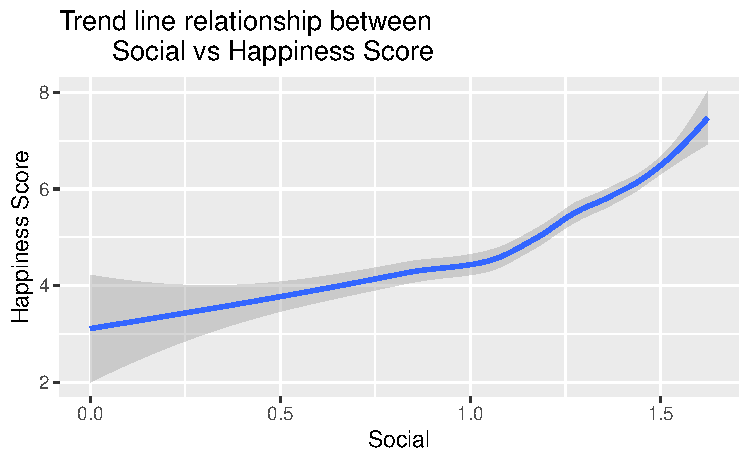
\includegraphics[width=0.7\linewidth]{Group_project_2_files/figure-latex/unnamed-chunk-10-1} \end{center}

\begin{Shaded}
\begin{Highlighting}[]
\NormalTok{data }\SpecialCharTok{\%\textgreater{}\%}
  \FunctionTok{ggplot}\NormalTok{() }\SpecialCharTok{+}
  \FunctionTok{geom\_smooth}\NormalTok{(}\AttributeTok{mapping =} \FunctionTok{aes}\NormalTok{(}\AttributeTok{x =}\NormalTok{ Health, }\AttributeTok{y =}\NormalTok{ Happiness\_Score)) }\SpecialCharTok{+}
  \FunctionTok{labs}\NormalTok{(}\AttributeTok{x =} \StringTok{"Health"}\NormalTok{, }\AttributeTok{y =} \StringTok{"Happiness Score"}\NormalTok{, }
       \AttributeTok{title=}\StringTok{"Trend line relationship between }
\StringTok{       Health vs Happiness Score"}\NormalTok{)}
\end{Highlighting}
\end{Shaded}

\begin{verbatim}
## `geom_smooth()` using method = 'loess' and formula = 'y ~ x'
\end{verbatim}

\begin{center}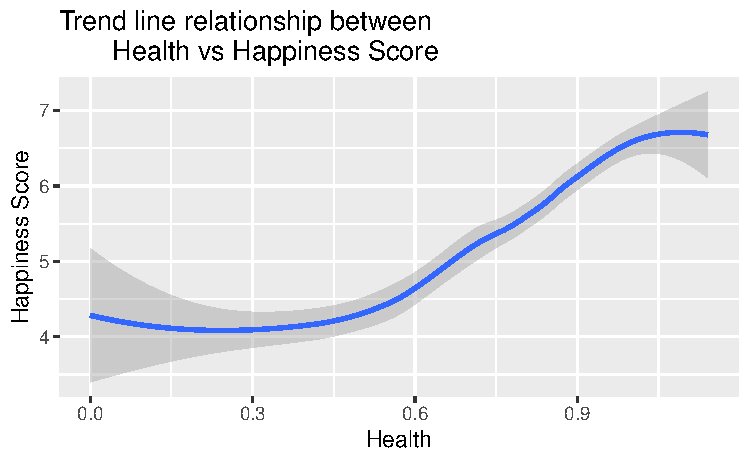
\includegraphics[width=0.7\linewidth]{Group_project_2_files/figure-latex/unnamed-chunk-11-1} \end{center}

\begin{Shaded}
\begin{Highlighting}[]
\NormalTok{data }\SpecialCharTok{\%\textgreater{}\%}
  \FunctionTok{ggplot}\NormalTok{() }\SpecialCharTok{+}
  \FunctionTok{geom\_smooth}\NormalTok{(}\AttributeTok{mapping =} \FunctionTok{aes}\NormalTok{(}\AttributeTok{x =}\NormalTok{ Freedom, }\AttributeTok{y =}\NormalTok{ Happiness\_Score)) }\SpecialCharTok{+}
  \FunctionTok{labs}\NormalTok{(}\AttributeTok{x =} \StringTok{"Freedom"}\NormalTok{, }\AttributeTok{y =} \StringTok{"Happiness Score"}\NormalTok{, }
       \AttributeTok{title=}\StringTok{"Trend line relationship between }
\StringTok{       Freedom vs Happiness Score"}\NormalTok{)}
\end{Highlighting}
\end{Shaded}

\begin{verbatim}
## `geom_smooth()` using method = 'loess' and formula = 'y ~ x'
\end{verbatim}

\begin{center}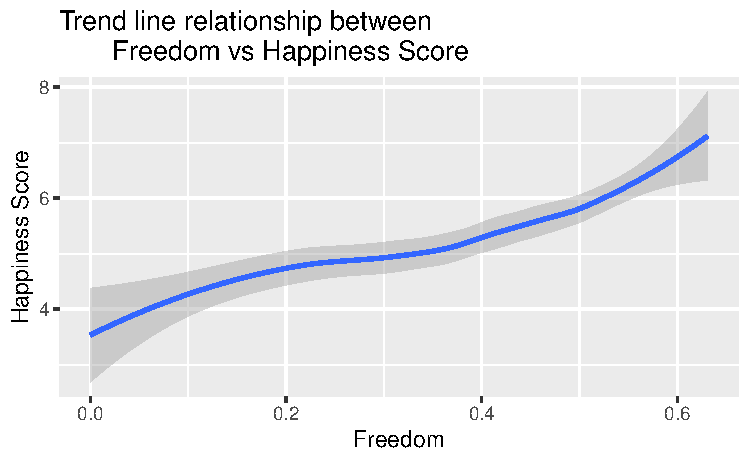
\includegraphics[width=0.7\linewidth]{Group_project_2_files/figure-latex/unnamed-chunk-12-1} \end{center}

\begin{Shaded}
\begin{Highlighting}[]
\NormalTok{data }\SpecialCharTok{\%\textgreater{}\%}
  \FunctionTok{ggplot}\NormalTok{() }\SpecialCharTok{+}
  \FunctionTok{geom\_smooth}\NormalTok{(}\AttributeTok{mapping =} \FunctionTok{aes}\NormalTok{(}\AttributeTok{x =}\NormalTok{ Corruption, }\AttributeTok{y =}\NormalTok{ Happiness\_Score)) }\SpecialCharTok{+}
  \FunctionTok{labs}\NormalTok{(}\AttributeTok{x =} \StringTok{"Corruption"}\NormalTok{, }\AttributeTok{y =} \StringTok{"Happiness Score"}\NormalTok{, }
       \AttributeTok{title=}\StringTok{"Trend line relationship between }
\StringTok{       Corruption vs Happiness Score"}\NormalTok{)}
\end{Highlighting}
\end{Shaded}

\begin{verbatim}
## `geom_smooth()` using method = 'loess' and formula = 'y ~ x'
\end{verbatim}

\begin{center}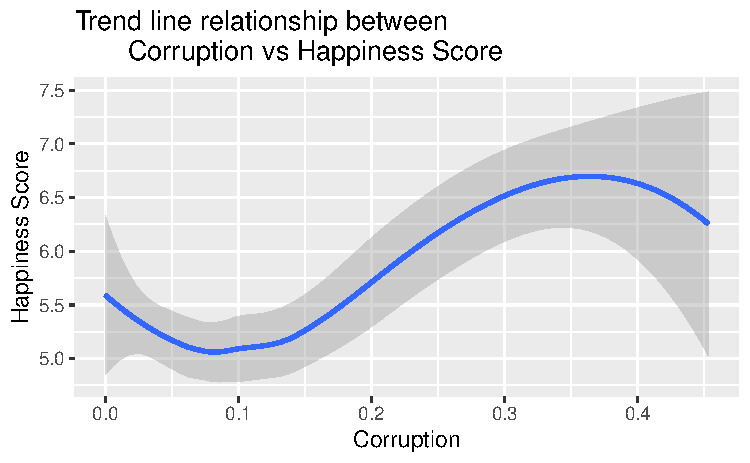
\includegraphics[width=0.7\linewidth]{Group_project_2_files/figure-latex/unnamed-chunk-13-1} \end{center}

*HeatMap

\begin{Shaded}
\begin{Highlighting}[]
\NormalTok{data }\SpecialCharTok{\%\textgreater{}\%}
\FunctionTok{ggplot}\NormalTok{(}\FunctionTok{aes}\NormalTok{(}\AttributeTok{x =}\NormalTok{ Economy, }\AttributeTok{y =}\NormalTok{ Happiness\_Score)) }\SpecialCharTok{+}
  \FunctionTok{geom\_bin2d}\NormalTok{(}\AttributeTok{bins =} \DecValTok{30}\NormalTok{) }\SpecialCharTok{+}  
  \FunctionTok{geom\_smooth}\NormalTok{(}\AttributeTok{method =} \StringTok{"lm"}\NormalTok{, }\AttributeTok{se =} \ConstantTok{FALSE}\NormalTok{) }\SpecialCharTok{+} 
  \FunctionTok{labs}\NormalTok{(}\AttributeTok{title =} \StringTok{"HeatMap with linearline }
\StringTok{                Economy vs Happiness Score"}\NormalTok{, }
           \AttributeTok{x =} \StringTok{"Economy"}\NormalTok{, }\AttributeTok{y =} \StringTok{"Happiness\_Score"}\NormalTok{)}
\end{Highlighting}
\end{Shaded}

\begin{verbatim}
## `geom_smooth()` using formula = 'y ~ x'
\end{verbatim}

\begin{center}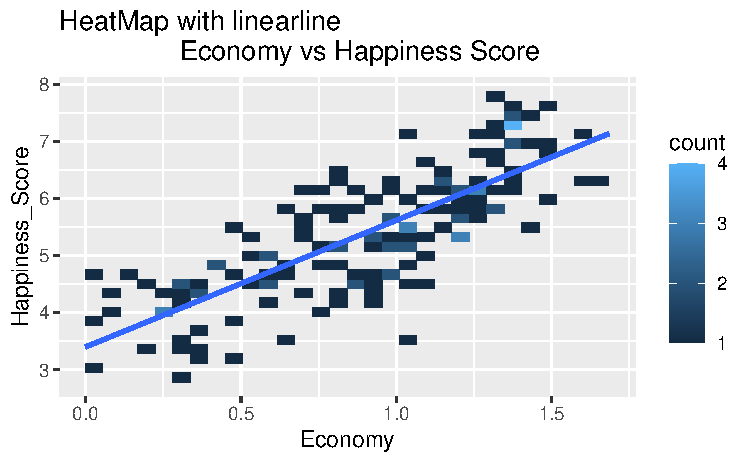
\includegraphics[width=0.7\linewidth]{Group_project_2_files/figure-latex/unnamed-chunk-14-1} \end{center}

\begin{Shaded}
\begin{Highlighting}[]
\NormalTok{data }\SpecialCharTok{\%\textgreater{}\%}
\FunctionTok{ggplot}\NormalTok{(}\FunctionTok{aes}\NormalTok{(}\AttributeTok{x =}\NormalTok{ Social, }\AttributeTok{y =}\NormalTok{ Happiness\_Score)) }\SpecialCharTok{+}
  \FunctionTok{geom\_bin2d}\NormalTok{(}\AttributeTok{bins =} \DecValTok{30}\NormalTok{) }\SpecialCharTok{+}  
  \FunctionTok{geom\_smooth}\NormalTok{(}\AttributeTok{method =} \StringTok{"lm"}\NormalTok{, }\AttributeTok{se =} \ConstantTok{FALSE}\NormalTok{) }\SpecialCharTok{+} 
  \FunctionTok{labs}\NormalTok{(}\AttributeTok{title =} \StringTok{"HeatMap with linearline }
\StringTok{                Social vs Happiness Score"}\NormalTok{, }
           \AttributeTok{x =} \StringTok{"Social"}\NormalTok{, }\AttributeTok{y =} \StringTok{"Happiness\_Score"}\NormalTok{)}
\end{Highlighting}
\end{Shaded}

\begin{verbatim}
## `geom_smooth()` using formula = 'y ~ x'
\end{verbatim}

\begin{center}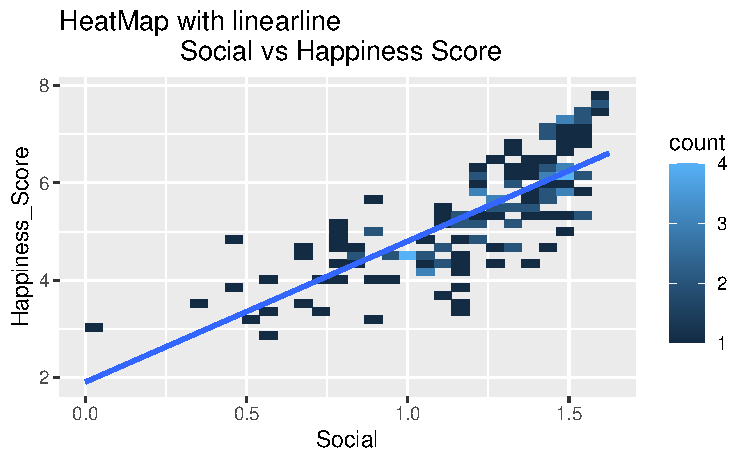
\includegraphics[width=0.7\linewidth]{Group_project_2_files/figure-latex/unnamed-chunk-15-1} \end{center}

\begin{Shaded}
\begin{Highlighting}[]
\NormalTok{data }\SpecialCharTok{\%\textgreater{}\%}
\FunctionTok{ggplot}\NormalTok{(}\FunctionTok{aes}\NormalTok{(}\AttributeTok{x =}\NormalTok{ Health, }\AttributeTok{y =}\NormalTok{ Happiness\_Score)) }\SpecialCharTok{+}
  \FunctionTok{geom\_bin2d}\NormalTok{(}\AttributeTok{bins =} \DecValTok{30}\NormalTok{) }\SpecialCharTok{+}  
  \FunctionTok{geom\_smooth}\NormalTok{(}\AttributeTok{method =} \StringTok{"lm"}\NormalTok{, }\AttributeTok{se =} \ConstantTok{FALSE}\NormalTok{) }\SpecialCharTok{+} 
  \FunctionTok{labs}\NormalTok{(}\AttributeTok{title =} \StringTok{"HeatMap with linearline }
\StringTok{                Health vs Happiness Score"}\NormalTok{, }
           \AttributeTok{x =} \StringTok{"Health"}\NormalTok{, }\AttributeTok{y =} \StringTok{"Happiness\_Score"}\NormalTok{)}
\end{Highlighting}
\end{Shaded}

\begin{verbatim}
## `geom_smooth()` using formula = 'y ~ x'
\end{verbatim}

\begin{center}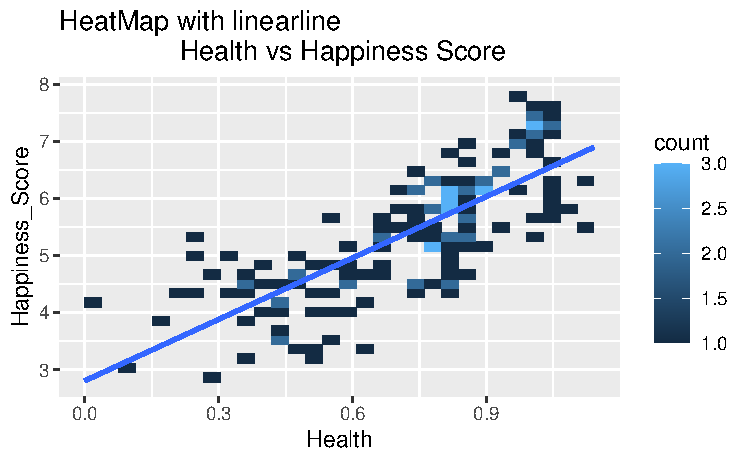
\includegraphics[width=0.7\linewidth]{Group_project_2_files/figure-latex/unnamed-chunk-16-1} \end{center}

\begin{Shaded}
\begin{Highlighting}[]
\NormalTok{data }\SpecialCharTok{\%\textgreater{}\%}
\FunctionTok{ggplot}\NormalTok{(}\FunctionTok{aes}\NormalTok{(}\AttributeTok{x =}\NormalTok{ Freedom, }\AttributeTok{y =}\NormalTok{ Happiness\_Score)) }\SpecialCharTok{+}
  \FunctionTok{geom\_bin2d}\NormalTok{(}\AttributeTok{bins =} \DecValTok{30}\NormalTok{) }\SpecialCharTok{+}  
  \FunctionTok{geom\_smooth}\NormalTok{(}\AttributeTok{method =} \StringTok{"lm"}\NormalTok{, }\AttributeTok{se =} \ConstantTok{FALSE}\NormalTok{) }\SpecialCharTok{+} 
  \FunctionTok{labs}\NormalTok{(}\AttributeTok{title =} \StringTok{"HeatMap with linearline }
\StringTok{                Freedom and Happiness Score"}\NormalTok{, }
           \AttributeTok{x =} \StringTok{"Freedom"}\NormalTok{, }\AttributeTok{y =} \StringTok{"Happiness\_Score"}\NormalTok{)}
\end{Highlighting}
\end{Shaded}

\begin{verbatim}
## `geom_smooth()` using formula = 'y ~ x'
\end{verbatim}

\begin{center}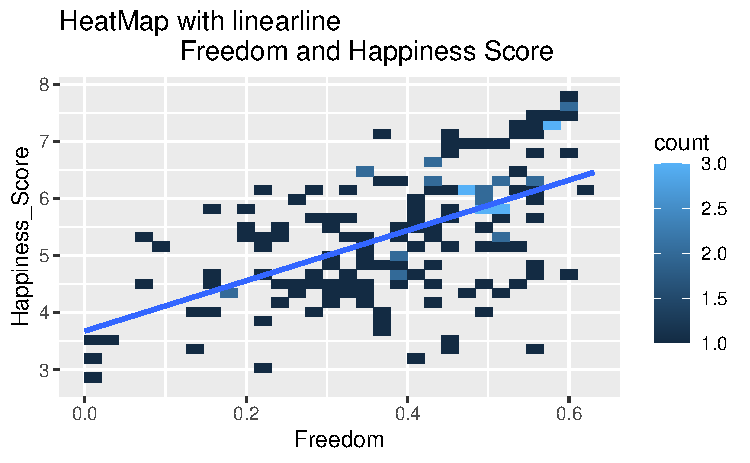
\includegraphics[width=0.7\linewidth]{Group_project_2_files/figure-latex/unnamed-chunk-17-1} \end{center}

\begin{Shaded}
\begin{Highlighting}[]
\NormalTok{data }\SpecialCharTok{\%\textgreater{}\%}
\FunctionTok{ggplot}\NormalTok{(}\FunctionTok{aes}\NormalTok{(}\AttributeTok{x =}\NormalTok{ Corruption, }\AttributeTok{y =}\NormalTok{ Happiness\_Score)) }\SpecialCharTok{+}
  \FunctionTok{geom\_bin2d}\NormalTok{(}\AttributeTok{bins =} \DecValTok{30}\NormalTok{) }\SpecialCharTok{+}  
  \FunctionTok{geom\_smooth}\NormalTok{(}\AttributeTok{method =} \StringTok{"lm"}\NormalTok{, }\AttributeTok{se =} \ConstantTok{FALSE}\NormalTok{) }\SpecialCharTok{+} 
  \FunctionTok{labs}\NormalTok{(}\AttributeTok{title =} \StringTok{"HeatMap with linearline}
\StringTok{                Corruption and Happiness Score"}\NormalTok{, }
           \AttributeTok{x =} \StringTok{"Corruption"}\NormalTok{, }\AttributeTok{y =} \StringTok{"Happiness\_Score"}\NormalTok{)}
\end{Highlighting}
\end{Shaded}

\begin{verbatim}
## `geom_smooth()` using formula = 'y ~ x'
\end{verbatim}

\begin{center}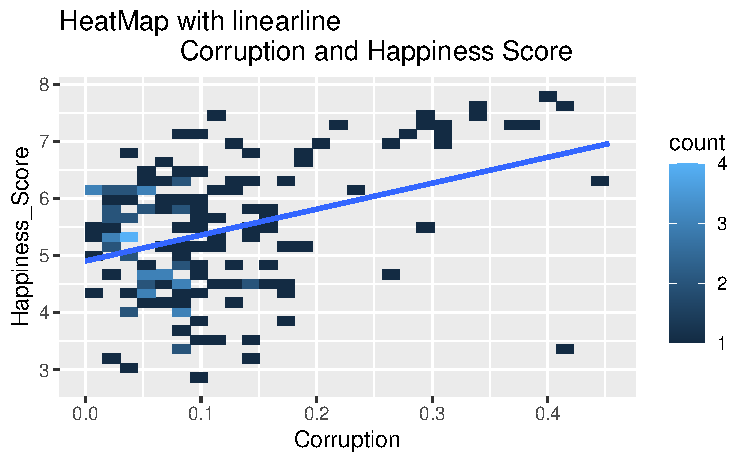
\includegraphics[width=0.7\linewidth]{Group_project_2_files/figure-latex/unnamed-chunk-18-1} \end{center}

======= {[} Module 4: Eugene Kim, Harold Lee - Explanatory Data Analysis
{]}

\begin{Shaded}
\begin{Highlighting}[]
\FunctionTok{str}\NormalTok{(data, }\AttributeTok{vec.len =} \DecValTok{2}\NormalTok{)}
\end{Highlighting}
\end{Shaded}

\begin{verbatim}
## tibble [156 x 9] (S3: tbl_df/tbl/data.frame)
##  $ Overall rank     : num [1:156] 1 2 3 4 5 ...
##  $ Country or region: chr [1:156] "Finland" "Denmark" ...
##  $ Happiness_Score  : num [1:156] 7.77 7.6 ...
##  $ Economy          : num [1:156] 1.34 1.38 ...
##  $ Social           : num [1:156] 1.59 1.57 ...
##  $ Health           : num [1:156] 0.986 0.996 ...
##  $ Freedom          : num [1:156] 0.596 0.592 0.603 0.591 0.557 ...
##  $ Generosity       : num [1:156] 0.153 0.252 0.271 0.354 0.322 ...
##  $ Corruption       : num [1:156] 0.393 0.41 0.341 0.118 0.298 ...
\end{verbatim}

\begin{Shaded}
\begin{Highlighting}[]
\FunctionTok{head}\NormalTok{(}
    \FunctionTok{select}\NormalTok{(data, Economy, Social, Health, Freedom, Corruption,}
\NormalTok{           Happiness\_Score)}
\NormalTok{  )}
\end{Highlighting}
\end{Shaded}

\begin{longtable}[]{@{}rrrrrr@{}}
\toprule\noalign{}
Economy & Social & Health & Freedom & Corruption & Happiness\_Score \\
\midrule\noalign{}
\endhead
\bottomrule\noalign{}
\endlastfoot
1.340 & 1.587 & 0.986 & 0.596 & 0.393 & 7.769 \\
1.383 & 1.573 & 0.996 & 0.592 & 0.410 & 7.600 \\
1.488 & 1.582 & 1.028 & 0.603 & 0.341 & 7.554 \\
1.380 & 1.624 & 1.026 & 0.591 & 0.118 & 7.494 \\
1.396 & 1.522 & 0.999 & 0.557 & 0.298 & 7.488 \\
1.452 & 1.526 & 1.052 & 0.572 & 0.343 & 7.480 \\
\end{longtable}

\begin{Shaded}
\begin{Highlighting}[]
\FunctionTok{tail}\NormalTok{(}\FunctionTok{select}\NormalTok{(data, Economy, Social, Health, Freedom, Corruption,}
\NormalTok{            Happiness\_Score)}
\NormalTok{  )}
\end{Highlighting}
\end{Shaded}

\begin{longtable}[]{@{}rrrrrr@{}}
\toprule\noalign{}
Economy & Social & Health & Freedom & Corruption & Happiness\_Score \\
\midrule\noalign{}
\endhead
\bottomrule\noalign{}
\endlastfoot
0.287 & 1.163 & 0.463 & 0.143 & 0.077 & 3.380 \\
0.359 & 0.711 & 0.614 & 0.555 & 0.411 & 3.334 \\
0.476 & 0.885 & 0.499 & 0.417 & 0.147 & 3.231 \\
0.350 & 0.517 & 0.361 & 0.000 & 0.025 & 3.203 \\
0.026 & 0.000 & 0.105 & 0.225 & 0.035 & 3.083 \\
0.306 & 0.575 & 0.295 & 0.010 & 0.091 & 2.853 \\
\end{longtable}

*Summary statistics

*Box Plot

\begin{Shaded}
\begin{Highlighting}[]
\NormalTok{data\_long }\OtherTok{\textless{}{-}}\NormalTok{ data }\SpecialCharTok{\%\textgreater{}\%}
  \FunctionTok{gather}\NormalTok{(}\AttributeTok{key =} \StringTok{"Variable"}\NormalTok{, }\AttributeTok{value =} \StringTok{"Score"}\NormalTok{, Economy, Social, Health,}
\NormalTok{         Freedom, Corruption) }

\FunctionTok{ggplot}\NormalTok{(data\_long, }\FunctionTok{aes}\NormalTok{(}\AttributeTok{x =}\NormalTok{ Variable, }\AttributeTok{y =}\NormalTok{ Score)) }\SpecialCharTok{+}
  \FunctionTok{geom\_boxplot}\NormalTok{(}\AttributeTok{width =} \FloatTok{0.7}\NormalTok{) }\SpecialCharTok{+} 
  \FunctionTok{theme}\NormalTok{(}\AttributeTok{axis.text.x =} \FunctionTok{element\_text}\NormalTok{(}\AttributeTok{angle =} \DecValTok{45}\NormalTok{, }\AttributeTok{hjust =} \DecValTok{1}\NormalTok{)) }\SpecialCharTok{+}
  \FunctionTok{labs}\NormalTok{(}\AttributeTok{title =} \StringTok{"Box Plot Each Variable"}\NormalTok{,}
       \AttributeTok{x =} \StringTok{"Variables Affecting Happiness Score"}\NormalTok{, }\AttributeTok{y =} \StringTok{"Values"}\NormalTok{)}
\end{Highlighting}
\end{Shaded}

\begin{center}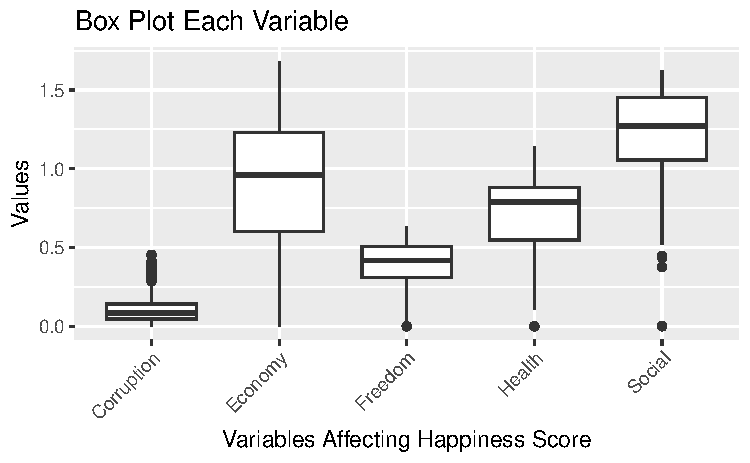
\includegraphics[width=0.7\linewidth]{Group_project_2_files/figure-latex/unnamed-chunk-20-1} \end{center}

*Violin Plot

\begin{Shaded}
\begin{Highlighting}[]
\FunctionTok{ggplot}\NormalTok{(data\_long, }\FunctionTok{aes}\NormalTok{(}\AttributeTok{x =}\NormalTok{ Variable, }\AttributeTok{y =}\NormalTok{ Score, }\AttributeTok{fill =}\NormalTok{ Variable)) }\SpecialCharTok{+}
  \FunctionTok{geom\_violin}\NormalTok{(}\AttributeTok{trim =} \ConstantTok{TRUE}\NormalTok{) }\SpecialCharTok{+} 
  \FunctionTok{theme}\NormalTok{(}\AttributeTok{axis.text.x =} \FunctionTok{element\_text}\NormalTok{(}\AttributeTok{angle =} \DecValTok{45}\NormalTok{, }\AttributeTok{hjust =} \DecValTok{1}\NormalTok{)) }\SpecialCharTok{+}
  \FunctionTok{labs}\NormalTok{(}\AttributeTok{title =} \StringTok{"Violin Plot of Each Variable"}\NormalTok{,}
       \AttributeTok{x =} \StringTok{"Variables Affecting Happiness Score"}\NormalTok{, }\AttributeTok{y =} \StringTok{"Values"}\NormalTok{) }\SpecialCharTok{+}
  \FunctionTok{scale\_fill\_brewer}\NormalTok{(}\AttributeTok{palette =} \StringTok{"Pastel1"}\NormalTok{)}
\end{Highlighting}
\end{Shaded}

\begin{center}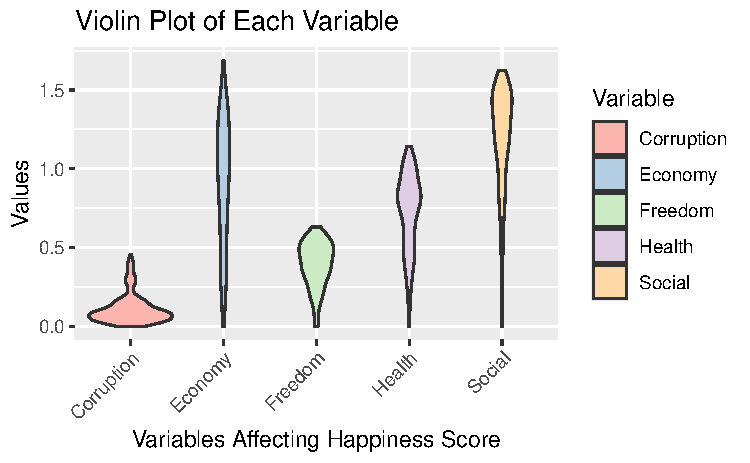
\includegraphics[width=0.7\linewidth]{Group_project_2_files/figure-latex/unnamed-chunk-21-1} \end{center}

*Summary

\begin{Shaded}
\begin{Highlighting}[]
\NormalTok{data }\SpecialCharTok{\%\textgreater{}\%}
  \FunctionTok{summarize}\NormalTok{(}
    \AttributeTok{mean=} \FunctionTok{mean}\NormalTok{(Economy),}
    \AttributeTok{median =} \FunctionTok{median}\NormalTok{(Economy),}
    \AttributeTok{sd =} \FunctionTok{sd}\NormalTok{(Economy),}
    \AttributeTok{iqr =} \FunctionTok{IQR}\NormalTok{(Economy),}
    \AttributeTok{min =} \FunctionTok{min}\NormalTok{(Economy),}
    \AttributeTok{max =} \FunctionTok{max}\NormalTok{(Economy)}
\NormalTok{ )}
\end{Highlighting}
\end{Shaded}

\begin{longtable}[]{@{}rrrrrr@{}}
\toprule\noalign{}
mean & median & sd & iqr & min & max \\
\midrule\noalign{}
\endhead
\bottomrule\noalign{}
\endlastfoot
0.9051474 & 0.96 & 0.3983895 & 0.62975 & 0 & 1.684 \\
\end{longtable}

\begin{Shaded}
\begin{Highlighting}[]
\NormalTok{data }\SpecialCharTok{\%\textgreater{}\%}
  \FunctionTok{summarize}\NormalTok{(}
    \AttributeTok{mean=} \FunctionTok{mean}\NormalTok{(Social),}
    \AttributeTok{median =} \FunctionTok{median}\NormalTok{(Social),}
    \AttributeTok{sd =} \FunctionTok{sd}\NormalTok{(Social),}
    \AttributeTok{iqr =} \FunctionTok{IQR}\NormalTok{(Social),}
    \AttributeTok{min =} \FunctionTok{min}\NormalTok{(Social),}
    \AttributeTok{max =} \FunctionTok{max}\NormalTok{(Social)}
\NormalTok{ )}
\end{Highlighting}
\end{Shaded}

\begin{longtable}[]{@{}rrrrrr@{}}
\toprule\noalign{}
mean & median & sd & iqr & min & max \\
\midrule\noalign{}
\endhead
\bottomrule\noalign{}
\endlastfoot
1.208814 & 1.2715 & 0.2991914 & 0.39675 & 0 & 1.624 \\
\end{longtable}

\begin{Shaded}
\begin{Highlighting}[]
\NormalTok{data }\SpecialCharTok{\%\textgreater{}\%}
  \FunctionTok{summarize}\NormalTok{(}
    \AttributeTok{mean=} \FunctionTok{mean}\NormalTok{(Health),}
    \AttributeTok{median =} \FunctionTok{median}\NormalTok{(Health),}
    \AttributeTok{sd =} \FunctionTok{sd}\NormalTok{(Health),}
    \AttributeTok{iqr =} \FunctionTok{IQR}\NormalTok{(Health),}
    \AttributeTok{min =} \FunctionTok{min}\NormalTok{(Health),}
    \AttributeTok{max =} \FunctionTok{max}\NormalTok{(Health)}
\NormalTok{ )}
\end{Highlighting}
\end{Shaded}

\begin{longtable}[]{@{}rrrrrr@{}}
\toprule\noalign{}
mean & median & sd & iqr & min & max \\
\midrule\noalign{}
\endhead
\bottomrule\noalign{}
\endlastfoot
0.7252436 & 0.789 & 0.242124 & 0.334 & 0 & 1.141 \\
\end{longtable}

\begin{Shaded}
\begin{Highlighting}[]
\NormalTok{data }\SpecialCharTok{\%\textgreater{}\%}
  \FunctionTok{summarize}\NormalTok{(}
    \AttributeTok{mean=} \FunctionTok{mean}\NormalTok{(Freedom),}
    \AttributeTok{median =} \FunctionTok{median}\NormalTok{(Freedom),}
    \AttributeTok{sd =} \FunctionTok{sd}\NormalTok{(Freedom),}
    \AttributeTok{iqr =} \FunctionTok{IQR}\NormalTok{(Freedom),}
    \AttributeTok{min =} \FunctionTok{min}\NormalTok{(Freedom),}
    \AttributeTok{max =} \FunctionTok{max}\NormalTok{(Freedom)}
\NormalTok{ )}
\end{Highlighting}
\end{Shaded}

\begin{longtable}[]{@{}rrrrrr@{}}
\toprule\noalign{}
mean & median & sd & iqr & min & max \\
\midrule\noalign{}
\endhead
\bottomrule\noalign{}
\endlastfoot
0.3925705 & 0.417 & 0.1432895 & 0.19925 & 0 & 0.631 \\
\end{longtable}

\begin{Shaded}
\begin{Highlighting}[]
\NormalTok{data }\SpecialCharTok{\%\textgreater{}\%}
  \FunctionTok{summarize}\NormalTok{(}
    \AttributeTok{mean=} \FunctionTok{mean}\NormalTok{(Corruption),}
    \AttributeTok{median =} \FunctionTok{median}\NormalTok{(Corruption),}
    \AttributeTok{sd =} \FunctionTok{sd}\NormalTok{(Corruption),}
    \AttributeTok{iqr =} \FunctionTok{IQR}\NormalTok{(Corruption),}
    \AttributeTok{min =} \FunctionTok{min}\NormalTok{(Corruption),}
    \AttributeTok{max =} \FunctionTok{max}\NormalTok{(Corruption)}
\NormalTok{ )}
\end{Highlighting}
\end{Shaded}

\begin{longtable}[]{@{}rrrrrr@{}}
\toprule\noalign{}
mean & median & sd & iqr & min & max \\
\midrule\noalign{}
\endhead
\bottomrule\noalign{}
\endlastfoot
0.1106026 & 0.0855 & 0.0945378 & 0.09425 & 0 & 0.453 \\
\end{longtable}

\begin{Shaded}
\begin{Highlighting}[]
\NormalTok{data\_E }\OtherTok{\textless{}{-}}\NormalTok{ data }\SpecialCharTok{\%\textgreater{}\%}
  \FunctionTok{summarize}\NormalTok{(}
    \AttributeTok{mean=} \FunctionTok{mean}\NormalTok{(Economy),}
    \AttributeTok{median =} \FunctionTok{median}\NormalTok{(Economy),}
    \AttributeTok{sd =} \FunctionTok{sd}\NormalTok{(Economy),}
    \AttributeTok{iqr =} \FunctionTok{IQR}\NormalTok{(Economy),}
    \AttributeTok{min =} \FunctionTok{min}\NormalTok{(Economy),}
    \AttributeTok{max =} \FunctionTok{max}\NormalTok{(Economy)}
\NormalTok{ )}
\end{Highlighting}
\end{Shaded}

\begin{Shaded}
\begin{Highlighting}[]
\NormalTok{data\_S }\OtherTok{\textless{}{-}}\NormalTok{ data }\SpecialCharTok{\%\textgreater{}\%}
  \FunctionTok{summarize}\NormalTok{(}
    \AttributeTok{mean=} \FunctionTok{mean}\NormalTok{(Social),}
    \AttributeTok{median =} \FunctionTok{median}\NormalTok{(Social),}
    \AttributeTok{sd =} \FunctionTok{sd}\NormalTok{(Social),}
    \AttributeTok{iqr =} \FunctionTok{IQR}\NormalTok{(Social),}
    \AttributeTok{min =} \FunctionTok{min}\NormalTok{(Social),}
    \AttributeTok{max =} \FunctionTok{max}\NormalTok{(Social)}
\NormalTok{ )}
\end{Highlighting}
\end{Shaded}

\begin{Shaded}
\begin{Highlighting}[]
\NormalTok{data\_H }\OtherTok{\textless{}{-}}\NormalTok{ data }\SpecialCharTok{\%\textgreater{}\%}
  \FunctionTok{summarize}\NormalTok{(}
    \AttributeTok{mean=} \FunctionTok{mean}\NormalTok{(Health),}
    \AttributeTok{median =} \FunctionTok{median}\NormalTok{(Health),}
    \AttributeTok{sd =} \FunctionTok{sd}\NormalTok{(Health),}
    \AttributeTok{iqr =} \FunctionTok{IQR}\NormalTok{(Health),}
    \AttributeTok{min =} \FunctionTok{min}\NormalTok{(Health),}
    \AttributeTok{max =} \FunctionTok{max}\NormalTok{(Health)}
\NormalTok{ )}
\end{Highlighting}
\end{Shaded}

\begin{Shaded}
\begin{Highlighting}[]
\NormalTok{data\_F }\OtherTok{\textless{}{-}}\NormalTok{ data }\SpecialCharTok{\%\textgreater{}\%}
  \FunctionTok{summarize}\NormalTok{(}
    \AttributeTok{mean=} \FunctionTok{mean}\NormalTok{(Freedom),}
    \AttributeTok{median =} \FunctionTok{median}\NormalTok{(Freedom),}
    \AttributeTok{sd =} \FunctionTok{sd}\NormalTok{(Freedom),}
    \AttributeTok{iqr =} \FunctionTok{IQR}\NormalTok{(Freedom),}
    \AttributeTok{min =} \FunctionTok{min}\NormalTok{(Freedom),}
    \AttributeTok{max =} \FunctionTok{max}\NormalTok{(Freedom)}
\NormalTok{ )}
\end{Highlighting}
\end{Shaded}

\begin{Shaded}
\begin{Highlighting}[]
\NormalTok{data\_C }\OtherTok{\textless{}{-}}\NormalTok{ data }\SpecialCharTok{\%\textgreater{}\%}
  \FunctionTok{summarize}\NormalTok{(}
    \AttributeTok{mean=} \FunctionTok{mean}\NormalTok{(Corruption),}
    \AttributeTok{median =} \FunctionTok{median}\NormalTok{(Corruption),}
    \AttributeTok{sd =} \FunctionTok{sd}\NormalTok{(Corruption),}
    \AttributeTok{iqr =} \FunctionTok{IQR}\NormalTok{(Corruption),}
    \AttributeTok{min =} \FunctionTok{min}\NormalTok{(Corruption),}
    \AttributeTok{max =} \FunctionTok{max}\NormalTok{(Corruption)}
\NormalTok{ )}
\end{Highlighting}
\end{Shaded}

\begin{Shaded}
\begin{Highlighting}[]
\NormalTok{combined\_data }\OtherTok{\textless{}{-}} \FunctionTok{rbind}\NormalTok{(data\_E, data\_S, data\_H, data\_F, data\_C)}
\end{Highlighting}
\end{Shaded}

\begin{Shaded}
\begin{Highlighting}[]
\NormalTok{combined\_data\_rounded }\OtherTok{\textless{}{-}}\NormalTok{ combined\_data }\SpecialCharTok{\%\textgreater{}\%}
  \FunctionTok{mutate}\NormalTok{(}\FunctionTok{across}\NormalTok{(}\FunctionTok{everything}\NormalTok{(), }\SpecialCharTok{\textasciitilde{}} \FunctionTok{round}\NormalTok{(., }\DecValTok{2}\NormalTok{)))}
\end{Highlighting}
\end{Shaded}

\begin{Shaded}
\begin{Highlighting}[]
\FunctionTok{row.names}\NormalTok{(combined\_data\_rounded) }\OtherTok{\textless{}{-}} \FunctionTok{c}\NormalTok{(}\StringTok{"Economy"}\NormalTok{, }\StringTok{"Social"}\NormalTok{, }\StringTok{"Health"}\NormalTok{,}\StringTok{"Freedom"}\NormalTok{, }\StringTok{"Corruption"}\NormalTok{)}
\end{Highlighting}
\end{Shaded}

\begin{verbatim}
## Warning: Setting row names on a tibble is deprecated.
\end{verbatim}

\begin{Shaded}
\begin{Highlighting}[]
\FunctionTok{print}\NormalTok{(combined\_data\_rounded)}
\end{Highlighting}
\end{Shaded}

\begin{verbatim}
## # A tibble: 5 x 6
##    mean median    sd   iqr   min   max
## * <dbl>  <dbl> <dbl> <dbl> <dbl> <dbl>
## 1  0.91   0.96  0.4   0.63     0  1.68
## 2  1.21   1.27  0.3   0.4      0  1.62
## 3  0.73   0.79  0.24  0.33     0  1.14
## 4  0.39   0.42  0.14  0.2      0  0.63
## 5  0.11   0.09  0.09  0.09     0  0.45
\end{verbatim}

\section{{[}Module 5: Chun Jin Park -
Modeling{]}.}\label{module-5-chun-jin-park---modeling.}

\section{Linear model using Im}\label{linear-model-using-im}

\begin{Shaded}
\begin{Highlighting}[]
\NormalTok{model }\OtherTok{\textless{}{-}} \FunctionTok{lm}\NormalTok{(Happiness\_Score }\SpecialCharTok{\textasciitilde{}}\NormalTok{ Economy }\SpecialCharTok{+}\NormalTok{ Social }\SpecialCharTok{+}\NormalTok{ Health }\SpecialCharTok{+}\NormalTok{ Freedom }\SpecialCharTok{+}\NormalTok{ Generosity}
            \SpecialCharTok{+}\NormalTok{ Corruption, }\AttributeTok{data =}\NormalTok{ data)}

\FunctionTok{summary}\NormalTok{(model)}
\end{Highlighting}
\end{Shaded}

\begin{verbatim}
## 
## Call:
## lm(formula = Happiness_Score ~ Economy + Social + Health + Freedom + 
##     Generosity + Corruption, data = data)
## 
## Residuals:
##      Min       1Q   Median       3Q      Max 
## -1.75304 -0.35306  0.05703  0.36695  1.19059 
## 
## Coefficients:
##             Estimate Std. Error t value Pr(>|t|)    
## (Intercept)   1.7952     0.2111   8.505 1.77e-14 ***
## Economy       0.7754     0.2182   3.553 0.000510 ***
## Social        1.1242     0.2369   4.745 4.83e-06 ***
## Health        1.0781     0.3345   3.223 0.001560 ** 
## Freedom       1.4548     0.3753   3.876 0.000159 ***
## Generosity    0.4898     0.4977   0.984 0.326709    
## Corruption    0.9723     0.5424   1.793 0.075053 .  
## ---
## Signif. codes:  0 '***' 0.001 '**' 0.01 '*' 0.05 '.' 0.1 ' ' 1
## 
## Residual standard error: 0.5335 on 149 degrees of freedom
## Multiple R-squared:  0.7792, Adjusted R-squared:  0.7703 
## F-statistic: 87.62 on 6 and 149 DF,  p-value: < 2.2e-16
\end{verbatim}

\section{Tidy to get the model
coefficients}\label{tidy-to-get-the-model-coefficients}

\begin{Shaded}
\begin{Highlighting}[]
\NormalTok{coefficients }\OtherTok{\textless{}{-}} \FunctionTok{tidy}\NormalTok{(model)}
\FunctionTok{print}\NormalTok{(coefficients)}
\end{Highlighting}
\end{Shaded}

\begin{verbatim}
## # A tibble: 7 x 5
##   term        estimate std.error statistic  p.value
##   <chr>          <dbl>     <dbl>     <dbl>    <dbl>
## 1 (Intercept)    1.80      0.211     8.51  1.77e-14
## 2 Economy        0.775     0.218     3.55  5.10e- 4
## 3 Social         1.12      0.237     4.75  4.83e- 6
## 4 Health         1.08      0.335     3.22  1.56e- 3
## 5 Freedom        1.45      0.375     3.88  1.59e- 4
## 6 Generosity     0.490     0.498     0.984 3.27e- 1
## 7 Corruption     0.972     0.542     1.79  7.51e- 2
\end{verbatim}

\section{Glance to get the model's performance
metrics}\label{glance-to-get-the-models-performance-metrics}

\begin{Shaded}
\begin{Highlighting}[]
\NormalTok{performance }\OtherTok{\textless{}{-}} \FunctionTok{glance}\NormalTok{(model)}
\FunctionTok{print}\NormalTok{(performance)}
\end{Highlighting}
\end{Shaded}

\begin{verbatim}
## # A tibble: 1 x 12
##   r.squared adj.r.squared sigma statistic  p.value    df logLik   AIC   BIC
##       <dbl>         <dbl> <dbl>     <dbl>    <dbl> <dbl>  <dbl> <dbl> <dbl>
## 1     0.779         0.770 0.534      87.6 2.40e-46     6  -120.  256.  280.
## # i 3 more variables: deviance <dbl>, df.residual <int>, nobs <int>
\end{verbatim}

\section{Observed vs Predicted plot}\label{observed-vs-predicted-plot}

\begin{Shaded}
\begin{Highlighting}[]
\FunctionTok{ggplot}\NormalTok{(data, }\FunctionTok{aes}\NormalTok{(}\AttributeTok{x =} \FunctionTok{predict}\NormalTok{(model), }\AttributeTok{y =}\NormalTok{ Happiness\_Score)) }\SpecialCharTok{+}
  \FunctionTok{geom\_point}\NormalTok{() }\SpecialCharTok{+}
  \FunctionTok{geom\_abline}\NormalTok{(}\AttributeTok{intercept =} \DecValTok{0}\NormalTok{, }\AttributeTok{slope =} \DecValTok{1}\NormalTok{, }\AttributeTok{col =} \StringTok{"red"}\NormalTok{) }\SpecialCharTok{+}
  \FunctionTok{labs}\NormalTok{(}\AttributeTok{title =} 
         \StringTok{"Observed vs Predicted Happiness Score"}\NormalTok{, }
       \AttributeTok{x =} \StringTok{"Predicted Happiness Score"}\NormalTok{, }
       \AttributeTok{y =} \StringTok{"Observed Happiness Score"}\NormalTok{)}
\end{Highlighting}
\end{Shaded}

\begin{center}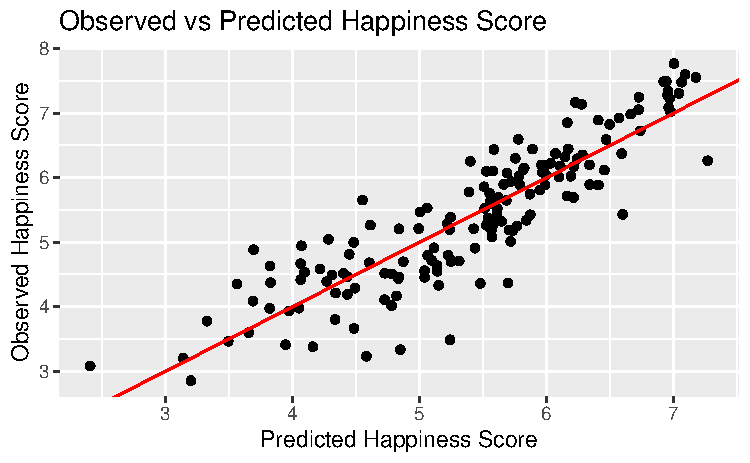
\includegraphics[width=0.7\linewidth]{Group_project_2_files/figure-latex/unnamed-chunk-38-1} \end{center}

\section{Residuals vs Predicted plot}\label{residuals-vs-predicted-plot}

\begin{Shaded}
\begin{Highlighting}[]
\FunctionTok{ggplot}\NormalTok{(data, }\FunctionTok{aes}\NormalTok{(}\AttributeTok{x =} \FunctionTok{predict}\NormalTok{(model), }\AttributeTok{y =} \FunctionTok{residuals}\NormalTok{(model))) }\SpecialCharTok{+}
  \FunctionTok{geom\_point}\NormalTok{() }\SpecialCharTok{+}
  \FunctionTok{geom\_hline}\NormalTok{(}\AttributeTok{yintercept =} \DecValTok{0}\NormalTok{, }\AttributeTok{col =} \StringTok{"red"}\NormalTok{) }\SpecialCharTok{+}
  \FunctionTok{labs}\NormalTok{(}\AttributeTok{title =} \StringTok{"Residuals vs Predicted Happiness Score"}\NormalTok{,}
       \AttributeTok{x =} \StringTok{"Predicted Happiness Score"}\NormalTok{, }
       \AttributeTok{y =} \StringTok{"Residuals"}\NormalTok{)}
\end{Highlighting}
\end{Shaded}

\begin{center}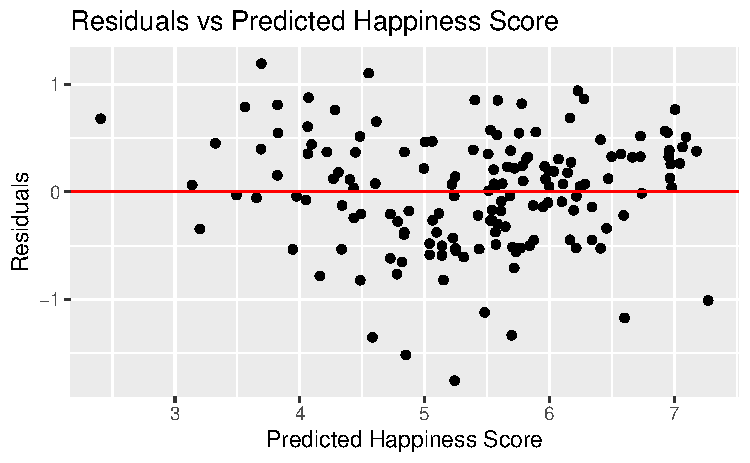
\includegraphics[width=0.7\linewidth]{Group_project_2_files/figure-latex/unnamed-chunk-39-1} \end{center}

\section{Q-Q plot}\label{q-q-plot}

\begin{Shaded}
\begin{Highlighting}[]
\FunctionTok{qqnorm}\NormalTok{(}\FunctionTok{residuals}\NormalTok{(model))}
\FunctionTok{qqline}\NormalTok{(}\FunctionTok{residuals}\NormalTok{(model), }\AttributeTok{col =} \StringTok{"red"}\NormalTok{)}
\end{Highlighting}
\end{Shaded}

\begin{center}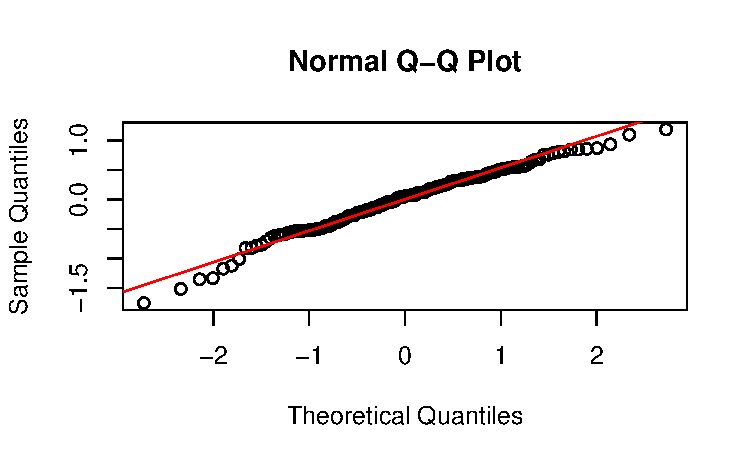
\includegraphics[width=0.7\linewidth]{Group_project_2_files/figure-latex/unnamed-chunk-40-1} \end{center}

\section{\textless\textless\textless\textless\textless\textless\textless{}
HEAD}\label{head}

{[}Module 6: Sena Julsdorf and Hyeongseok Sim{]}

\begin{Shaded}
\begin{Highlighting}[]
\FunctionTok{ggplot}\NormalTok{(data, }\FunctionTok{aes}\NormalTok{(}\AttributeTok{x =}\NormalTok{ Economy, }\AttributeTok{y =}\NormalTok{ Happiness\_Score)) }\SpecialCharTok{+}
  \FunctionTok{geom\_point}\NormalTok{() }\SpecialCharTok{+}
  \FunctionTok{geom\_smooth}\NormalTok{(}\AttributeTok{method =} \StringTok{"lm"}\NormalTok{, }\AttributeTok{se =} \ConstantTok{FALSE}\NormalTok{, }\AttributeTok{col =} \StringTok{"blue"}\NormalTok{) }\SpecialCharTok{+}
  \FunctionTok{labs}\NormalTok{(}\AttributeTok{title =} \StringTok{"Scatter Plot of Happiness Score based on Economy"}\NormalTok{, }
       \AttributeTok{x =} \StringTok{"Economic Score"}\NormalTok{, }
       \AttributeTok{y =} \StringTok{"Happiness Score"}\NormalTok{)}
\end{Highlighting}
\end{Shaded}

\begin{verbatim}
## `geom_smooth()` using formula = 'y ~ x'
\end{verbatim}

\begin{center}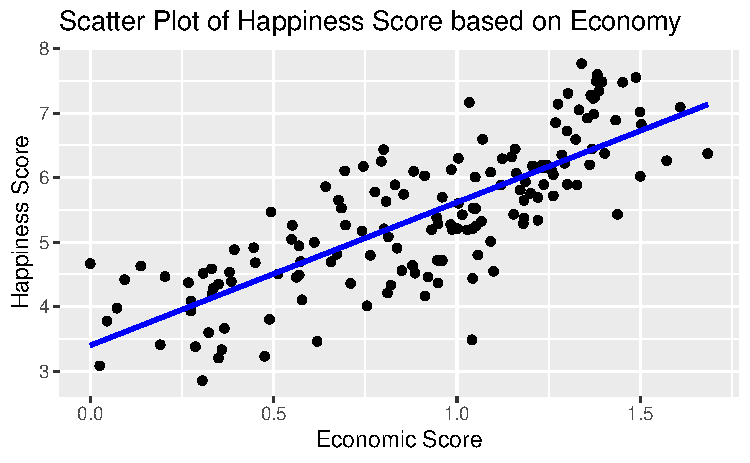
\includegraphics[width=0.7\linewidth]{Group_project_2_files/figure-latex/unnamed-chunk-41-1} \end{center}

\begin{Shaded}
\begin{Highlighting}[]
\FunctionTok{library}\NormalTok{(ggplot2)}
\FunctionTok{library}\NormalTok{(caTools)}
\end{Highlighting}
\end{Shaded}

\begin{Shaded}
\begin{Highlighting}[]
\FunctionTok{set.seed}\NormalTok{(}\DecValTok{123}\NormalTok{)}
\NormalTok{split }\OtherTok{\textless{}{-}} \FunctionTok{sample.split}\NormalTok{(data}\SpecialCharTok{$}\NormalTok{Happiness\_Score, }\AttributeTok{SplitRatio =} \FloatTok{0.5}\NormalTok{)}
\NormalTok{training\_set }\OtherTok{\textless{}{-}} \FunctionTok{subset}\NormalTok{(data, split }\SpecialCharTok{==} \ConstantTok{TRUE}\NormalTok{)}
\NormalTok{testing\_set }\OtherTok{\textless{}{-}} \FunctionTok{subset}\NormalTok{(data, split }\SpecialCharTok{==} \ConstantTok{FALSE}\NormalTok{)}
\end{Highlighting}
\end{Shaded}

\begin{Shaded}
\begin{Highlighting}[]
\NormalTok{lmmodel }\OtherTok{\textless{}{-}} \FunctionTok{lm}\NormalTok{(Happiness\_Score }\SpecialCharTok{\textasciitilde{}}\NormalTok{ Economy, }\AttributeTok{data =}\NormalTok{ testing\_set)}
\FunctionTok{summary}\NormalTok{(lmmodel)}
\end{Highlighting}
\end{Shaded}

\begin{verbatim}
## 
## Call:
## lm(formula = Happiness_Score ~ Economy, data = testing_set)
## 
## Residuals:
##      Min       1Q   Median       3Q      Max 
## -1.30817 -0.49891  0.02652  0.50746  1.27935 
## 
## Coefficients:
##             Estimate Std. Error t value Pr(>|t|)    
## (Intercept)   3.2913     0.2002   16.44   <2e-16 ***
## Economy       2.3317     0.1974   11.81   <2e-16 ***
## ---
## Signif. codes:  0 '***' 0.001 '**' 0.01 '*' 0.05 '.' 0.1 ' ' 1
## 
## Residual standard error: 0.6552 on 76 degrees of freedom
## Multiple R-squared:  0.6474, Adjusted R-squared:  0.6428 
## F-statistic: 139.6 on 1 and 76 DF,  p-value: < 2.2e-16
\end{verbatim}

\begin{Shaded}
\begin{Highlighting}[]
\NormalTok{predictions }\OtherTok{\textless{}{-}} \FunctionTok{predict}\NormalTok{(lmmodel, }\AttributeTok{newdata =}\NormalTok{ testing\_set)}
\end{Highlighting}
\end{Shaded}

\begin{Shaded}
\begin{Highlighting}[]
\NormalTok{rmse }\OtherTok{\textless{}{-}} \FunctionTok{sqrt}\NormalTok{(}\FunctionTok{mean}\NormalTok{((testing\_set}\SpecialCharTok{$}\NormalTok{Happiness\_Score }\SpecialCharTok{{-}}\NormalTok{ predictions)}\SpecialCharTok{\^{}}\DecValTok{2}\NormalTok{))}
\FunctionTok{print}\NormalTok{(}\FunctionTok{paste}\NormalTok{(}\StringTok{"RMSE: "}\NormalTok{, rmse))}
\end{Highlighting}
\end{Shaded}

\begin{verbatim}
## [1] "RMSE:  0.646727299146686"
\end{verbatim}

\begin{Shaded}
\begin{Highlighting}[]
\NormalTok{r\_squared }\OtherTok{\textless{}{-}} \FunctionTok{summary}\NormalTok{(lmmodel)}\SpecialCharTok{$}\NormalTok{r.squared}
\FunctionTok{print}\NormalTok{(}\FunctionTok{paste}\NormalTok{(}\StringTok{"R{-}squared: "}\NormalTok{, r\_squared))}
\end{Highlighting}
\end{Shaded}

\begin{verbatim}
## [1] "R-squared:  0.647436919488881"
\end{verbatim}

\begin{Shaded}
\begin{Highlighting}[]
\FunctionTok{ggplot}\NormalTok{(data, }\FunctionTok{aes}\NormalTok{(}\AttributeTok{x =}\NormalTok{ Social, }\AttributeTok{y =}\NormalTok{ Happiness\_Score)) }\SpecialCharTok{+}
  \FunctionTok{geom\_point}\NormalTok{() }\SpecialCharTok{+}
  \FunctionTok{geom\_smooth}\NormalTok{(}\AttributeTok{method =} \StringTok{"lm"}\NormalTok{, }\AttributeTok{se =} \ConstantTok{FALSE}\NormalTok{, }\AttributeTok{col =} \StringTok{"blue"}\NormalTok{) }\SpecialCharTok{+}
  \FunctionTok{labs}\NormalTok{(}\AttributeTok{title =} \StringTok{"Scatter Plot of Happiness Score based on Social"}\NormalTok{, }
       \AttributeTok{x =} \StringTok{"Social Score"}\NormalTok{, }
       \AttributeTok{y =} \StringTok{"Happiness Score"}\NormalTok{)}
\end{Highlighting}
\end{Shaded}

\begin{verbatim}
## `geom_smooth()` using formula = 'y ~ x'
\end{verbatim}

\begin{center}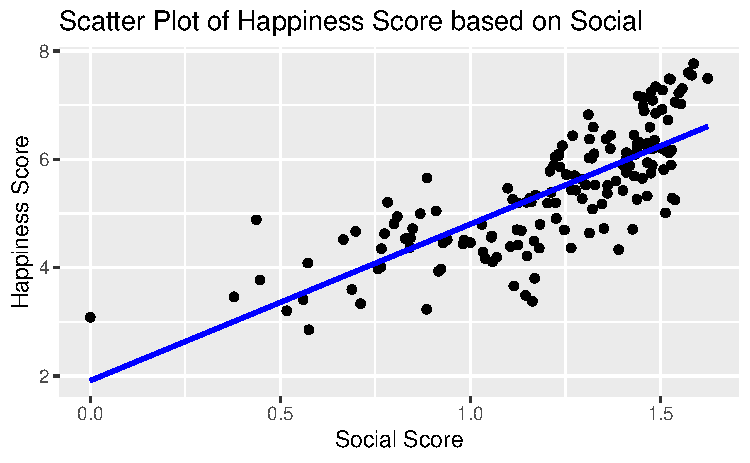
\includegraphics[width=0.7\linewidth]{Group_project_2_files/figure-latex/unnamed-chunk-48-1} \end{center}

\begin{Shaded}
\begin{Highlighting}[]
\NormalTok{lmmodel\_2 }\OtherTok{\textless{}{-}} \FunctionTok{lm}\NormalTok{(Happiness\_Score }\SpecialCharTok{\textasciitilde{}}\NormalTok{ Social, }\AttributeTok{data =}\NormalTok{ testing\_set)}
\FunctionTok{summary}\NormalTok{(lmmodel\_2)}
\end{Highlighting}
\end{Shaded}

\begin{verbatim}
## 
## Call:
## lm(formula = Happiness_Score ~ Social, data = testing_set)
## 
## Residuals:
##      Min       1Q   Median       3Q      Max 
## -1.91246 -0.50723  0.04253  0.55227  1.19156 
## 
## Coefficients:
##             Estimate Std. Error t value Pr(>|t|)    
## (Intercept)   1.8034     0.3742   4.819 7.23e-06 ***
## Social        3.0001     0.2974  10.089 1.13e-15 ***
## ---
## Signif. codes:  0 '***' 0.001 '**' 0.01 '*' 0.05 '.' 0.1 ' ' 1
## 
## Residual standard error: 0.7214 on 76 degrees of freedom
## Multiple R-squared:  0.5725, Adjusted R-squared:  0.5669 
## F-statistic: 101.8 on 1 and 76 DF,  p-value: 1.128e-15
\end{verbatim}

\begin{Shaded}
\begin{Highlighting}[]
\NormalTok{predictions\_2 }\OtherTok{\textless{}{-}} \FunctionTok{predict}\NormalTok{(lmmodel\_2, }\AttributeTok{newdata =}\NormalTok{ testing\_set)}
\end{Highlighting}
\end{Shaded}

\begin{Shaded}
\begin{Highlighting}[]
\NormalTok{rmse\_2 }\OtherTok{\textless{}{-}} \FunctionTok{sqrt}\NormalTok{(}\FunctionTok{mean}\NormalTok{((testing\_set}\SpecialCharTok{$}\NormalTok{Happiness\_Score }\SpecialCharTok{{-}}\NormalTok{ predictions\_2)}\SpecialCharTok{\^{}}\DecValTok{2}\NormalTok{))}
\FunctionTok{print}\NormalTok{(}\FunctionTok{paste}\NormalTok{(}\StringTok{"RMSE (Social model): "}\NormalTok{, rmse\_2))}
\end{Highlighting}
\end{Shaded}

\begin{verbatim}
## [1] "RMSE (Social model):  0.712139313572519"
\end{verbatim}

\begin{Shaded}
\begin{Highlighting}[]
\NormalTok{r\_squared\_2 }\OtherTok{\textless{}{-}} \FunctionTok{summary}\NormalTok{(lmmodel\_2)}\SpecialCharTok{$}\NormalTok{r.squared}
\FunctionTok{print}\NormalTok{(}\FunctionTok{paste}\NormalTok{(}\StringTok{"R{-}squared (Social model): "}\NormalTok{, r\_squared\_2))}
\end{Highlighting}
\end{Shaded}

\begin{verbatim}
## [1] "R-squared (Social model):  0.57251156656046"
\end{verbatim}

\begin{Shaded}
\begin{Highlighting}[]
\FunctionTok{ggplot}\NormalTok{(data, }\FunctionTok{aes}\NormalTok{(}\AttributeTok{x =}\NormalTok{ Freedom, }\AttributeTok{y =}\NormalTok{ Happiness\_Score)) }\SpecialCharTok{+}
  \FunctionTok{geom\_point}\NormalTok{() }\SpecialCharTok{+}
  \FunctionTok{geom\_smooth}\NormalTok{(}\AttributeTok{method =} \StringTok{"lm"}\NormalTok{, }\AttributeTok{se =} \ConstantTok{FALSE}\NormalTok{, }\AttributeTok{col =} \StringTok{"blue"}\NormalTok{) }\SpecialCharTok{+}
  \FunctionTok{labs}\NormalTok{(}\AttributeTok{title =} \StringTok{"Scatter Plot of Happiness Score based on Freedom"}\NormalTok{, }
       \AttributeTok{x =} \StringTok{"Freedom Score"}\NormalTok{, }
       \AttributeTok{y =} \StringTok{"Happiness Score"}\NormalTok{)}
\end{Highlighting}
\end{Shaded}

\begin{verbatim}
## `geom_smooth()` using formula = 'y ~ x'
\end{verbatim}

\begin{center}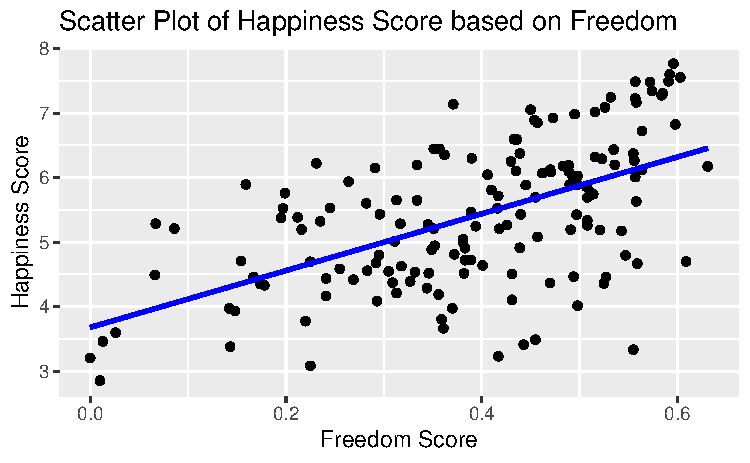
\includegraphics[width=0.7\linewidth]{Group_project_2_files/figure-latex/unnamed-chunk-53-1} \end{center}

\begin{Shaded}
\begin{Highlighting}[]
\NormalTok{lmmodel\_3 }\OtherTok{\textless{}{-}} \FunctionTok{lm}\NormalTok{(Happiness\_Score }\SpecialCharTok{\textasciitilde{}}\NormalTok{ Freedom, }\AttributeTok{data =}\NormalTok{ testing\_set)}
\FunctionTok{summary}\NormalTok{(lmmodel\_3)}
\end{Highlighting}
\end{Shaded}

\begin{verbatim}
## 
## Call:
## lm(formula = Happiness_Score ~ Freedom, data = testing_set)
## 
## Residuals:
##     Min      1Q  Median      3Q     Max 
## -2.8451 -0.6640 -0.0348  0.8907  1.7633 
## 
## Coefficients:
##             Estimate Std. Error t value Pr(>|t|)    
## (Intercept)   3.7556     0.3318  11.317  < 2e-16 ***
## Freedom       4.3667     0.7930   5.507 4.77e-07 ***
## ---
## Signif. codes:  0 '***' 0.001 '**' 0.01 '*' 0.05 '.' 0.1 ' ' 1
## 
## Residual standard error: 0.9329 on 76 degrees of freedom
## Multiple R-squared:  0.2852, Adjusted R-squared:  0.2758 
## F-statistic: 30.32 on 1 and 76 DF,  p-value: 4.768e-07
\end{verbatim}

\begin{Shaded}
\begin{Highlighting}[]
\NormalTok{predictions\_3 }\OtherTok{\textless{}{-}} \FunctionTok{predict}\NormalTok{(lmmodel\_3, }\AttributeTok{newdata =}\NormalTok{ testing\_set)}
\end{Highlighting}
\end{Shaded}

\begin{Shaded}
\begin{Highlighting}[]
\NormalTok{rmse\_3 }\OtherTok{\textless{}{-}} \FunctionTok{sqrt}\NormalTok{(}\FunctionTok{mean}\NormalTok{((testing\_set}\SpecialCharTok{$}\NormalTok{Happiness\_Score }\SpecialCharTok{{-}}\NormalTok{ predictions\_3)}\SpecialCharTok{\^{}}\DecValTok{2}\NormalTok{))}
\FunctionTok{print}\NormalTok{(}\FunctionTok{paste}\NormalTok{(}\StringTok{"RMSE (Freedom model): "}\NormalTok{, rmse\_3))}
\end{Highlighting}
\end{Shaded}

\begin{verbatim}
## [1] "RMSE (Freedom model):  0.920858315286326"
\end{verbatim}

\begin{Shaded}
\begin{Highlighting}[]
\NormalTok{r\_squared\_3 }\OtherTok{\textless{}{-}} \FunctionTok{summary}\NormalTok{(lmmodel\_3)}\SpecialCharTok{$}\NormalTok{r.squared}
\FunctionTok{print}\NormalTok{(}\FunctionTok{paste}\NormalTok{(}\StringTok{"R{-}squared (Freedom model): "}\NormalTok{, r\_squared\_3))}
\end{Highlighting}
\end{Shaded}

\begin{verbatim}
## [1] "R-squared (Freedom model):  0.285207357638025"
\end{verbatim}

\begin{Shaded}
\begin{Highlighting}[]
\FunctionTok{ggplot}\NormalTok{(data, }\FunctionTok{aes}\NormalTok{(}\AttributeTok{x =}\NormalTok{ Health, }\AttributeTok{y =}\NormalTok{ Happiness\_Score)) }\SpecialCharTok{+}
  \FunctionTok{geom\_point}\NormalTok{() }\SpecialCharTok{+}
  \FunctionTok{geom\_smooth}\NormalTok{(}\AttributeTok{method =} \StringTok{"lm"}\NormalTok{, }\AttributeTok{se =} \ConstantTok{FALSE}\NormalTok{, }\AttributeTok{col =} \StringTok{"blue"}\NormalTok{) }\SpecialCharTok{+}
  \FunctionTok{labs}\NormalTok{(}\AttributeTok{title =} \StringTok{"Scatter Plot of Happiness Score based on Health"}\NormalTok{, }
       \AttributeTok{x =} \StringTok{"Health Score"}\NormalTok{, }
       \AttributeTok{y =} \StringTok{"Happiness Score"}\NormalTok{)}
\end{Highlighting}
\end{Shaded}

\begin{verbatim}
## `geom_smooth()` using formula = 'y ~ x'
\end{verbatim}

\begin{center}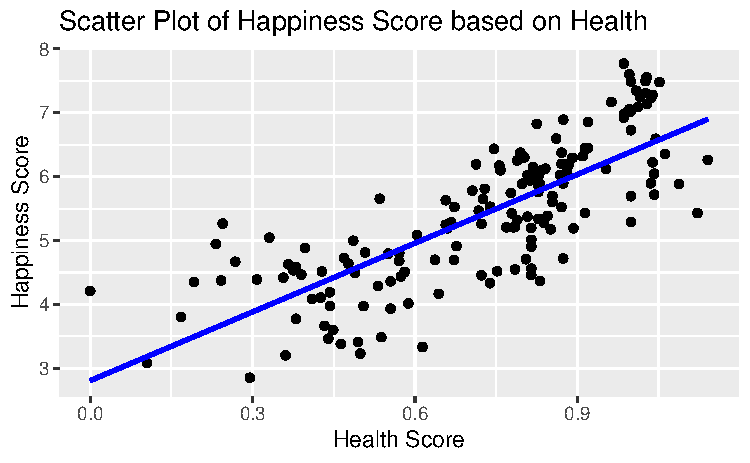
\includegraphics[width=0.7\linewidth]{Group_project_2_files/figure-latex/unnamed-chunk-58-1} \end{center}

\begin{Shaded}
\begin{Highlighting}[]
\NormalTok{lmmodel\_4 }\OtherTok{\textless{}{-}} \FunctionTok{lm}\NormalTok{(Happiness\_Score }\SpecialCharTok{\textasciitilde{}}\NormalTok{ Health, }\AttributeTok{data =}\NormalTok{ testing\_set)}
\FunctionTok{summary}\NormalTok{(lmmodel\_4)}
\end{Highlighting}
\end{Shaded}

\begin{verbatim}
## 
## Call:
## lm(formula = Happiness_Score ~ Health, data = testing_set)
## 
## Residuals:
##      Min       1Q   Median       3Q      Max 
## -1.64520 -0.40654  0.06847  0.54871  1.50718 
## 
## Coefficients:
##             Estimate Std. Error t value Pr(>|t|)    
## (Intercept)   2.7048     0.2762   9.794 4.08e-15 ***
## Health        3.7042     0.3519  10.525  < 2e-16 ***
## ---
## Signif. codes:  0 '***' 0.001 '**' 0.01 '*' 0.05 '.' 0.1 ' ' 1
## 
## Residual standard error: 0.7039 on 76 degrees of freedom
## Multiple R-squared:  0.5931, Adjusted R-squared:  0.5878 
## F-statistic: 110.8 on 1 and 76 DF,  p-value: < 2.2e-16
\end{verbatim}

\begin{Shaded}
\begin{Highlighting}[]
\NormalTok{predictions\_4 }\OtherTok{\textless{}{-}} \FunctionTok{predict}\NormalTok{(lmmodel\_4, }\AttributeTok{newdata =}\NormalTok{ testing\_set)}
\end{Highlighting}
\end{Shaded}

\begin{Shaded}
\begin{Highlighting}[]
\NormalTok{rmse\_4 }\OtherTok{\textless{}{-}} \FunctionTok{sqrt}\NormalTok{(}\FunctionTok{mean}\NormalTok{((testing\_set}\SpecialCharTok{$}\NormalTok{Happiness\_Score }\SpecialCharTok{{-}}\NormalTok{ predictions\_4)}\SpecialCharTok{\^{}}\DecValTok{2}\NormalTok{))}
\FunctionTok{print}\NormalTok{(}\FunctionTok{paste}\NormalTok{(}\StringTok{"RMSE (Health model): "}\NormalTok{, rmse\_4))}
\end{Highlighting}
\end{Shaded}

\begin{verbatim}
## [1] "RMSE (Health model):  0.694771303098578"
\end{verbatim}

\begin{Shaded}
\begin{Highlighting}[]
\NormalTok{r\_squared\_4 }\OtherTok{\textless{}{-}} \FunctionTok{summary}\NormalTok{(lmmodel\_4)}\SpecialCharTok{$}\NormalTok{r.squared}
\FunctionTok{print}\NormalTok{(}\FunctionTok{paste}\NormalTok{(}\StringTok{"R{-}squared (Health model): "}\NormalTok{, r\_squared\_4))}
\end{Highlighting}
\end{Shaded}

\begin{verbatim}
## [1] "R-squared (Health model):  0.593108901180756"
\end{verbatim}

\begin{Shaded}
\begin{Highlighting}[]
\NormalTok{lmmodel\_5 }\OtherTok{\textless{}{-}} \FunctionTok{lm}\NormalTok{(Happiness\_Score }\SpecialCharTok{\textasciitilde{}}\NormalTok{ Economy, }\AttributeTok{data =}\NormalTok{ training\_set)}
\FunctionTok{summary}\NormalTok{(lmmodel\_5)}
\end{Highlighting}
\end{Shaded}

\begin{verbatim}
## 
## Call:
## lm(formula = Happiness_Score ~ Economy, data = training_set)
## 
## Residuals:
##      Min       1Q   Median       3Q      Max 
## -2.20542 -0.45196  0.01283  0.52414  1.48846 
## 
## Coefficients:
##             Estimate Std. Error t value Pr(>|t|)    
## (Intercept)   3.4813     0.1863   18.68   <2e-16 ***
## Economy       2.1250     0.1937   10.97   <2e-16 ***
## ---
## Signif. codes:  0 '***' 0.001 '**' 0.01 '*' 0.05 '.' 0.1 ' ' 1
## 
## Residual standard error: 0.7083 on 76 degrees of freedom
## Multiple R-squared:  0.6129, Adjusted R-squared:  0.6078 
## F-statistic: 120.3 on 1 and 76 DF,  p-value: < 2.2e-16
\end{verbatim}

\begin{Shaded}
\begin{Highlighting}[]
\NormalTok{predictions\_5 }\OtherTok{\textless{}{-}} \FunctionTok{predict}\NormalTok{(lmmodel, }\AttributeTok{newdata =}\NormalTok{ training\_set)}
\end{Highlighting}
\end{Shaded}

\begin{Shaded}
\begin{Highlighting}[]
\NormalTok{rmse\_5 }\OtherTok{\textless{}{-}} \FunctionTok{sqrt}\NormalTok{(}\FunctionTok{mean}\NormalTok{((testing\_set}\SpecialCharTok{$}\NormalTok{Happiness\_Score }\SpecialCharTok{{-}}\NormalTok{ predictions\_5)}\SpecialCharTok{\^{}}\DecValTok{2}\NormalTok{))}
\FunctionTok{print}\NormalTok{(}\FunctionTok{paste}\NormalTok{(}\StringTok{"RMSE: "}\NormalTok{, rmse))}
\end{Highlighting}
\end{Shaded}

\begin{verbatim}
## [1] "RMSE:  0.646727299146686"
\end{verbatim}

\begin{Shaded}
\begin{Highlighting}[]
\NormalTok{r\_squared\_5 }\OtherTok{\textless{}{-}} \FunctionTok{summary}\NormalTok{(lmmodel\_5)}\SpecialCharTok{$}\NormalTok{r.squared}
\end{Highlighting}
\end{Shaded}

\begin{Shaded}
\begin{Highlighting}[]
\FunctionTok{print}\NormalTok{(}\FunctionTok{paste}\NormalTok{(}\StringTok{"R{-}squared (Economy model): "}\NormalTok{, r\_squared\_5))}
\end{Highlighting}
\end{Shaded}

\begin{verbatim}
## [1] "R-squared (Economy model):  0.612897269110227"
\end{verbatim}

\end{document}
